\documentclass{report}

% Page Size
\usepackage[letterpaper, portrait, margin=1in, left=1.5in]{geometry}

% Spacing
\usepackage{setspace}
\setlength{\parskip}{\baselineskip}
\doublespacing{}


% Bibliography
\usepackage[american]{babel}
\usepackage[style=apa, citestyle=apa, backend=biber]{biblatex}
\DeclareLanguageMapping{american}{american-apa}
\addbibresource{references.bib}
\usepackage[babel,threshold=2]{csquotes}

% Graphics
\usepackage{graphicx}
\graphicspath{ {./images/} }

% Table of Content
\setcounter{tocdepth}{2}

% Code Formatting
\usepackage{minted}
\usemintedstyle{pastie}

\def\code#1{\texttt{#1}}

% Positioning
\usepackage{float}

% Acronyms
\usepackage{acro}

\DeclareAcronym{iso}{
	short=ISO,
	long=International Organization for Standardization
}

\DeclareAcronym{ansi}{
	short=ANSI,
	long=American National Standards Institute
}

\DeclareAcronym{jis}{
	short=JIS,
	long=Japanese International Standards
}

\DeclareAcronym{wpm}{
	short=WPM,
	long=Words per Minute
}

\DeclareAcronym{neck}{
	short=WRNULD,
	long=Work-related neck and upper limb disorders
}

\DeclareAcronym{cv}{
	short=CV,
	long=Computer Vision
}

% Chapter Formatting
\usepackage{titlesec}
\titleformat{\chapter}[display]
{\centering\LARGE\normalfont\bfseries}
{Chapter \thechapter}
{0em}
{\vspace{-1.5ex}}

% Colors
\usepackage[dvipsnames]{xcolor}

% Links
\usepackage{hyperref}
\hypersetup{
	pdftitle={Development of a touch typing trainer with an emphasis on finger and wrist placement},
	pdfstartview={FitH},
	colorlinks=true,
	linkcolor=black,
	citecolor=black,
	filecolor=black,
	urlcolor=MidnightBlue
}

% Misc
\usepackage{gensymb}
\usepackage{amsmath}

%Flowchart
\usepackage{tikz}
\usetikzlibrary{shapes,positioning,calc}

% Adjust Figure Spacing
\setlength\intextsep{1cm}

\begin{document}

\pagenumbering{gobble}
\begin{titlepage}
	\centering

	\hspace{0pt}
	\vfill

	
\includegraphics[width=0.2\textwidth]{upc.png}
	
\includegraphics[width=0.2\textwidth]{dcs.png}
	\par\vspace{1cm}

	\textsc{Development of a touch typing trainer\\with an emphasis on finger and wrist positions}
	\par\vspace{0.5cm}

	\hrulefill
	\par\vspace{0.25cm}
	A Special Project Proposal Presented to the\\
	Faculty of the Department of Computer Science,\\
	University of the Philippines Cebu

	\par\vspace{0.25cm}
	In Partial Fulfillment\\
	Of the Requirements for the Degree\\
	Bachelor of Science in Computer Science\\
	\par\vspace{0.25cm}
	\hrulefill
	\par\vspace{0.5cm}

	Oscar Vian L. Valles\\
	BS Computer Science
	\par\vspace{0.5cm}

	Dhong Fhel K. Gom-os\\
	Adviser
	\par\vspace{0.5cm}

	October 2021
	\vfill
	\hspace{0pt}
\end{titlepage}
\newpage


\printacronyms
\newpage

\tableofcontents
\newpage

\pagenumbering{arabic}

\chapter{Introduction}


%FIXME - Lots of passive voice
\section{Background of the Study}
There are a lot of educational typing tests available that help people learn
touch typing, including Monkeytype, TypeRacer, and Keybr. These typing tests list
out words that are then typed out. The inputted keys are then compared to check
if the user has typed the expected letter. At the end of the test, the time
taken is calculated, and certain metrics are given. These metrics include words
per minute (WPM) and accuracy \parencite{bartnik2021}.

However, this method of examination leaves out a crucial part of typing —
ergonomics. Ergonomic typing prevents a lot of health issues in the future like
repetitive strain injury or carpal tunnel. One important factor that affects
ergonomics is the typing procedure and posture. This means the proper placement of
the wrist, hands, and hitting the keys using the right finger that is assigned
to the key.

Correct finger placement is usually taught at the beginning using a diagram,
with each key being associated with a specific finger. For instance, the letter
Q in a QWERTY layout should be hit using the fifth digit of the left hand, and
this is shown by coloring the fifth digit and the key Q with the same color or
by placing the letters directly on the fingers \parencite{dobson2009touch}.

Incorrect finger placement may cause these hand and wrist positions: ulnar
deviation, forearm pronation, and wrist extension \parencite{serina1999}. These
three are hand and wrist positions that are common in all activities, however,
prolonged periods in these positions may cause injuries such as Carpal
tunnel syndrome (CTS) \parencite{toosi2015}

In addition, this type of typing is frequently taught in the beginner level
\parencite{donica2018}. This means that there is a need to weed out bad habits
that may develop, like using the index finger for pressing the spacebar or
backspace. However, it is impractical for an educator to check each student if
they are not performing these movements as these may only show for a small
period which may not be caught in time.

Thus, there is a need for automatically detecting which finger is used during
typing, and for the position of the wrist in relation to the arm. One way to do
this is through finger and hand tracking. One solution for tracking is by using
image processing and machine learning. An example of this is MediaPipe
by~\cite{mediapipe}.

MediaPipe allows for various applications for machine learning in the field of
image processing. This includes, hand tracking, pose estimation, object
detection, and others. Another example of a library that allows for hand and
finger tracking is OpenCV by~\cite{opencv}. This is a tool that simplifies
computer vision and image processing. Machine learning can also be used with
OpenCV.

\section{Research Objectives}

\subsection{General Objectives}
To create a touch typing trainer that detects poor finger placement and hand
position to help develop better typing habits and healthier typing ergonomics.

\subsection{Specific Objectives}
\begin{itemize}
	\item To develop a program that tracks fingers and hand positions while typing
	\item To create a subroutine that ascertains which finger was used to type a key
	\item To detect if incorrect fingers were used to press a key or if the
	      position of the hand in relation to the wrist is problematic
	\item To assess the accuracy and performance of the developed program's ability
	      to perform the previously stated objectives
	\item To develop a user-friendly interface for users to train touch typing
	      using the developed program
	\item To generate key statistics of a user's touch typing performance:
	      \begin{itemize}
		      \item Words per Minute
		      \item Accuracy
		      \item Finger Placement Accuracy
	      \end{itemize}
\end{itemize}


\section{Scope and Limitation}
This research will focus on typing on a 60\% keyboard. Figure~\ref{fig:60}
illustrates this type of keyboard. This type of keyboard only has the
alphanumeric part of the keyboard. This limits the number of keys to be checked
and the expected movement of the hand. Furthermore, the keycaps will also be of
a light color, while the surface that the keyboard rests upon will be of a dark
color.

In addition, the keyboard layout will be \ac{ansi}. This layout is described by the
American National Standards Institute \parencite{ansi}. This is the most
common layout in the United States. However, it is also used in numerous
English-speaking countries such as the Philippines, Malaysia, and India.

The program will expect the that user has all ten digits and has no hand,
finger, or wrist deformities. In addition, only the placement of the hands,
fingers, and wrists will be taken into account when determining if the
ergonomics of the user while typing is healthy. The program will not check
seating position, angle of elbows, and other metrics for an ergonomic typing
posture while typing.

Capturing of the video to be analyzed by the program would be limited to a
single 480p webcam that is capturing in 24 frames per second. The camera will
be pointed downwards facing the keyboard and the hand. This means that the
vertical angle of the wrist may not be accurate.

\begin{figure}[H]
	\centering
	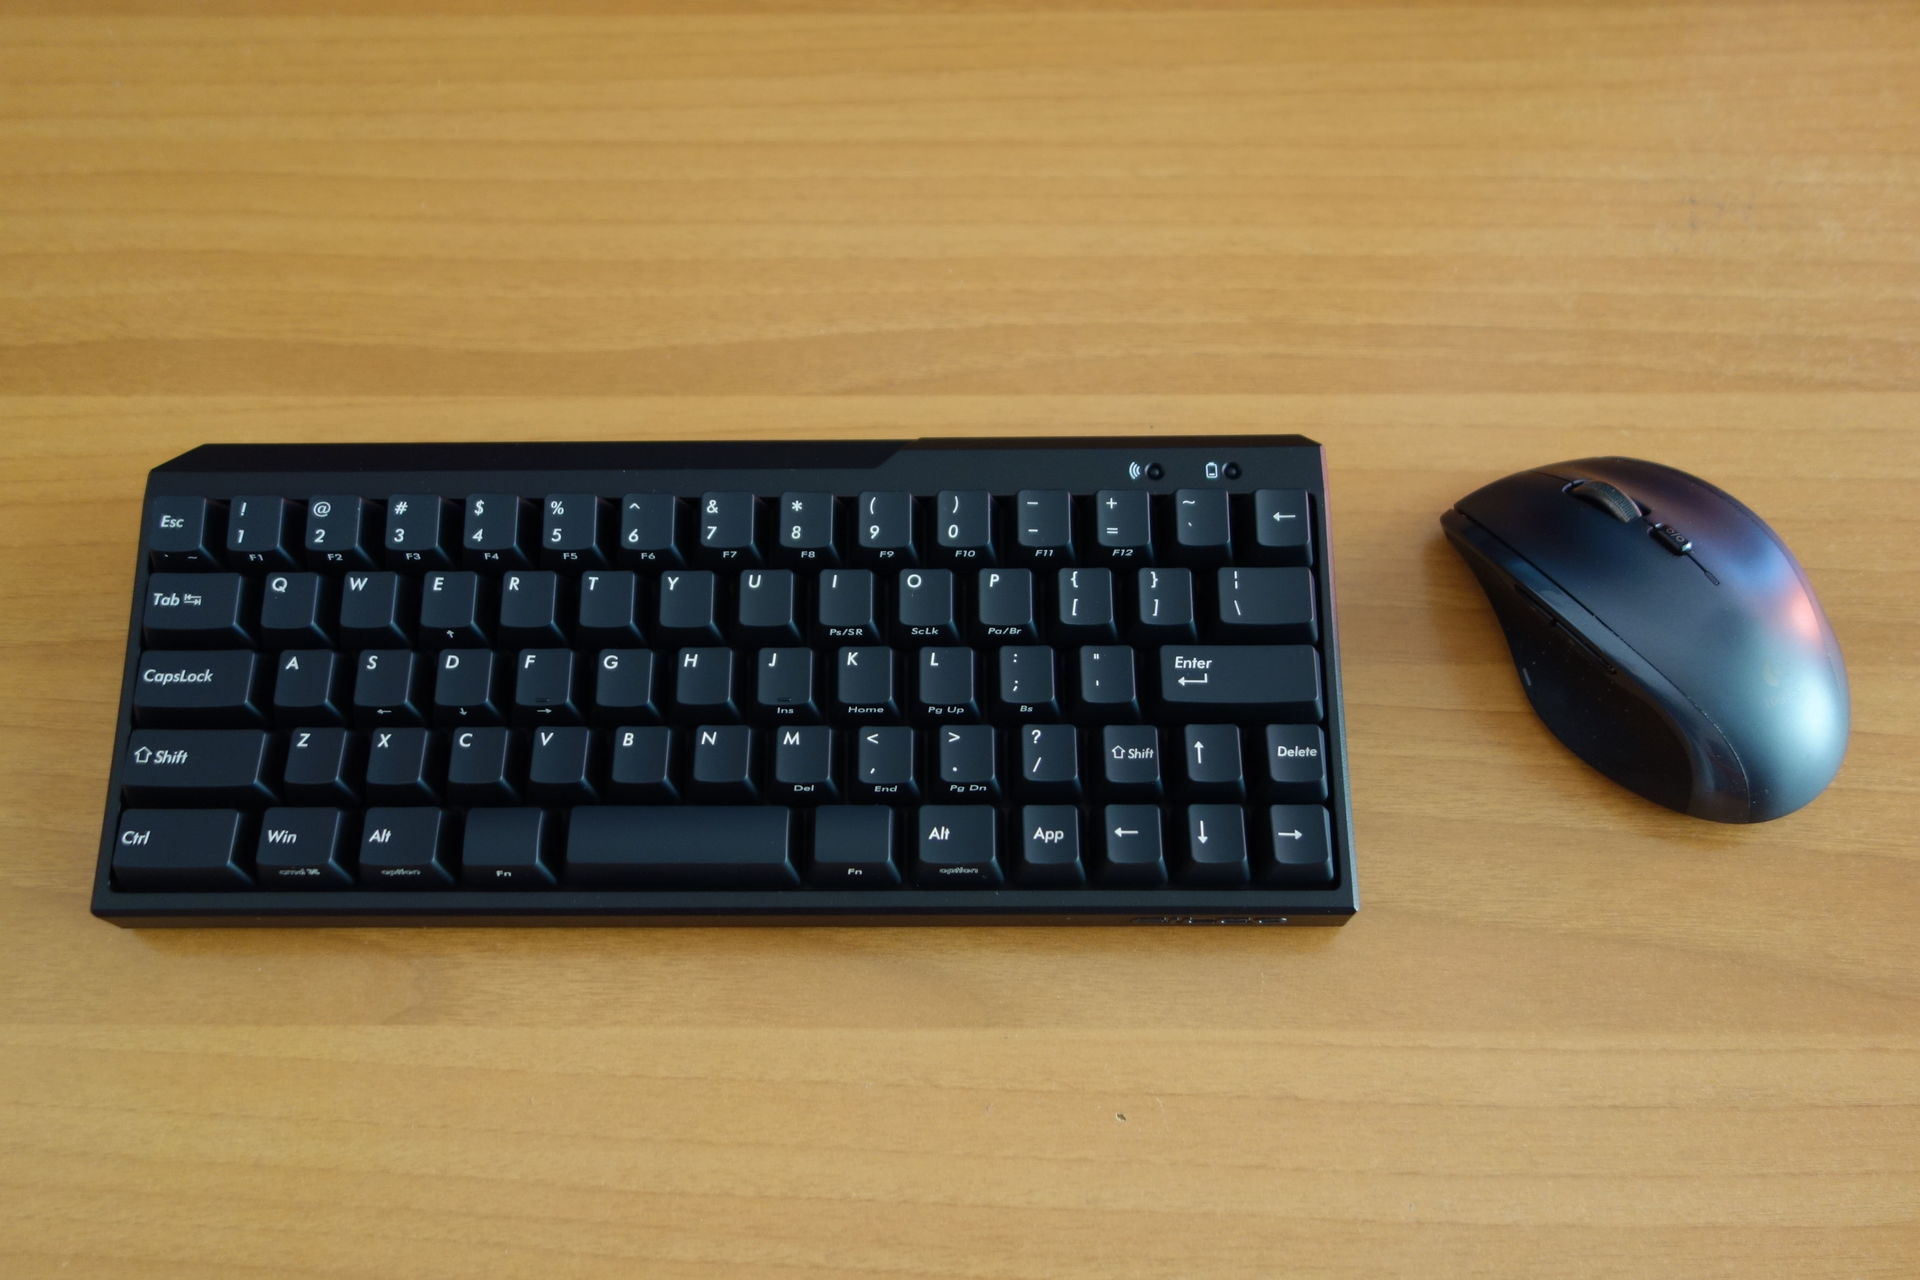
\includegraphics[width=0.8\textwidth]{60.jpg}
	\caption{A 60\% keyboard in \ac{ansi} layout. Reprinted from \fullcite{60}}
	\label{fig:60}
	\centering
\end{figure}


\section{Significance of the Research}
This research is beneficial for all users of physical keyboards. These include a
vast majority of the population as there are a lot of professions that heavily
rely on keyboards. Examples include developers, physicians, educators,
accountants. By having better ergonomics while typing, wrist injuries can be
prevented, and typing speed may be increased

This research also helps educators, especially early educators teaching beginner
typists. By automatically checking for ergonomics, posture, and correct
technique, the burden of checking each student is lessened, and directed
interventions for bad habits can be easily created as students with these bad
habits are easily identified

This research has a direct impact on people that has hand or wrist injuries that
are caused by poor typing habits. By correcting these poor habits, pain from
these injuries will be lessened, and even be prevented from occurring in the
first place. A specific example of this is by reducing ulnar deviation which
affects the nerve that is indicative of CTS \parencite{toosi2015}.

\chapter{Preliminary Review of Related Literature}

\section{Keyboard Typing}

Keyboard typing is the process of using a keyboard to input characters in a
system. In the context of this paper, keyboard typing will refer to the act of
using a physical keyboard to input characters in a computer system.

% Insert more about keyboard typing here %

\subsection{Keyboard Layouts and Form Factors}

One key characteristic of a keyboard is its physical attributes. Keyboards come
in a lot of layouts and form factors. Keyboard layouts are the shapes, size, and
positions of a key on a keyboard while the form factor of a keyboard refers to
its shape and dimensions. The form factor also refers to the number of keys included
in the keyboard \parencite{parkkinen2018}. By combining different layouts and
form factors, different permutations of a keyboard can be created.

Different keyboard layouts and form factors also produce different effects for
the user. This is due to how vastly different some keyboard layouts and form
factors are from one another. Some layouts focus on ergonomics, while others
focus on typing speed. Some form factors were designed for aesthetics, while
others focus on comfort and health. As such, different layouts may affect typing
performance, ergonomics, and long-term health effects \parencite{ciobanu2015}.

\subsubsection{ANSI and ISO Layout}

There are two common keyboard layouts around the world --- \ac{iso} and \ac{ansi}.

\citeauthor{ansi} is the standard that first defined the \ac{ansi} layout.
Figure~\ref{fig:ansi} illustrates what the \ac{ansi} layout looks like. This layout
is also used by countries other than America. Examples of countries that use
this layout as its standard is the Philippines, China, and Korea
\parencite{apple-layout}. However, these countries also opt to modify the layout
by adding extra layers to accommodate other character sets.

\citeauthor{iso} is the standard series that defines a framework that is used to
create other layouts. Layouts created from this standard are colloquially called
\ac{iso} Layouts. Countries around the world use this framework to create layouts
that fit the characters in their language. Examples of countries that use this
framework to create their own layout are France, Greece, Canada, and Sweden
\parencite{apple-layout}.

Both of these layouts usually utilize the same key ordering. This ordering is
commonly called QWERTY, based on the first five characters of the first row
of this specific layout.

There are other layouts available, however, they are not as common as the two
previously mentioned layouts. Examples of this include \ac{jis}. Other esoteric
layouts, like Tsangan or split-backspace, also exist. These layouts modify the
\ac{iso} and \ac{ansi} standards by adding or removing certain keys to fit the
character set of a language, or for additional keys. Other layouts are also
exactly the same as \ac{ansi} or \ac{iso}, however, these layouts change the
arrangement of the alphabet within the keyboard.

Despite the ubiquity of these common layouts, studies have shown that these
layouts are not ergonomic. The main issue with these layouts is the random
configurations of the letters. The randomness of the layout necessitates
memorization of the layout which reduces the ease of learning, reduces performance
in typing by reducing speed, and increases of typing errors
\parencite{ciobanu2015}.

\subsubsection{Keyboard Form Factors}

There is only one common keyboard form factor used worldwide: the full-size
keyboard. This keyboard contains all the keys specified in the keyboard
layout. This includes the alphanumeric keys, the function keys, the navigation
cluster, and the numpad.

Other common keyboard form factors are based on the full-size keyboard. The name
of these layouts, 60\%, 75\%, and 80\% reference the remaining number of keys
after cutting a portion off from the full-size keyboard. The 60\% keyboards only
contain the alphanumeric cluster while the 80\% and 75\% layouts retain the
navigation cluster and the function keys \parencite{parkkinen2018}. The main
draw for using keyboards with reduced sizes is for aesthetics, space
constraints, and ergonomics.

\begin{figure}[H]
	\centering
	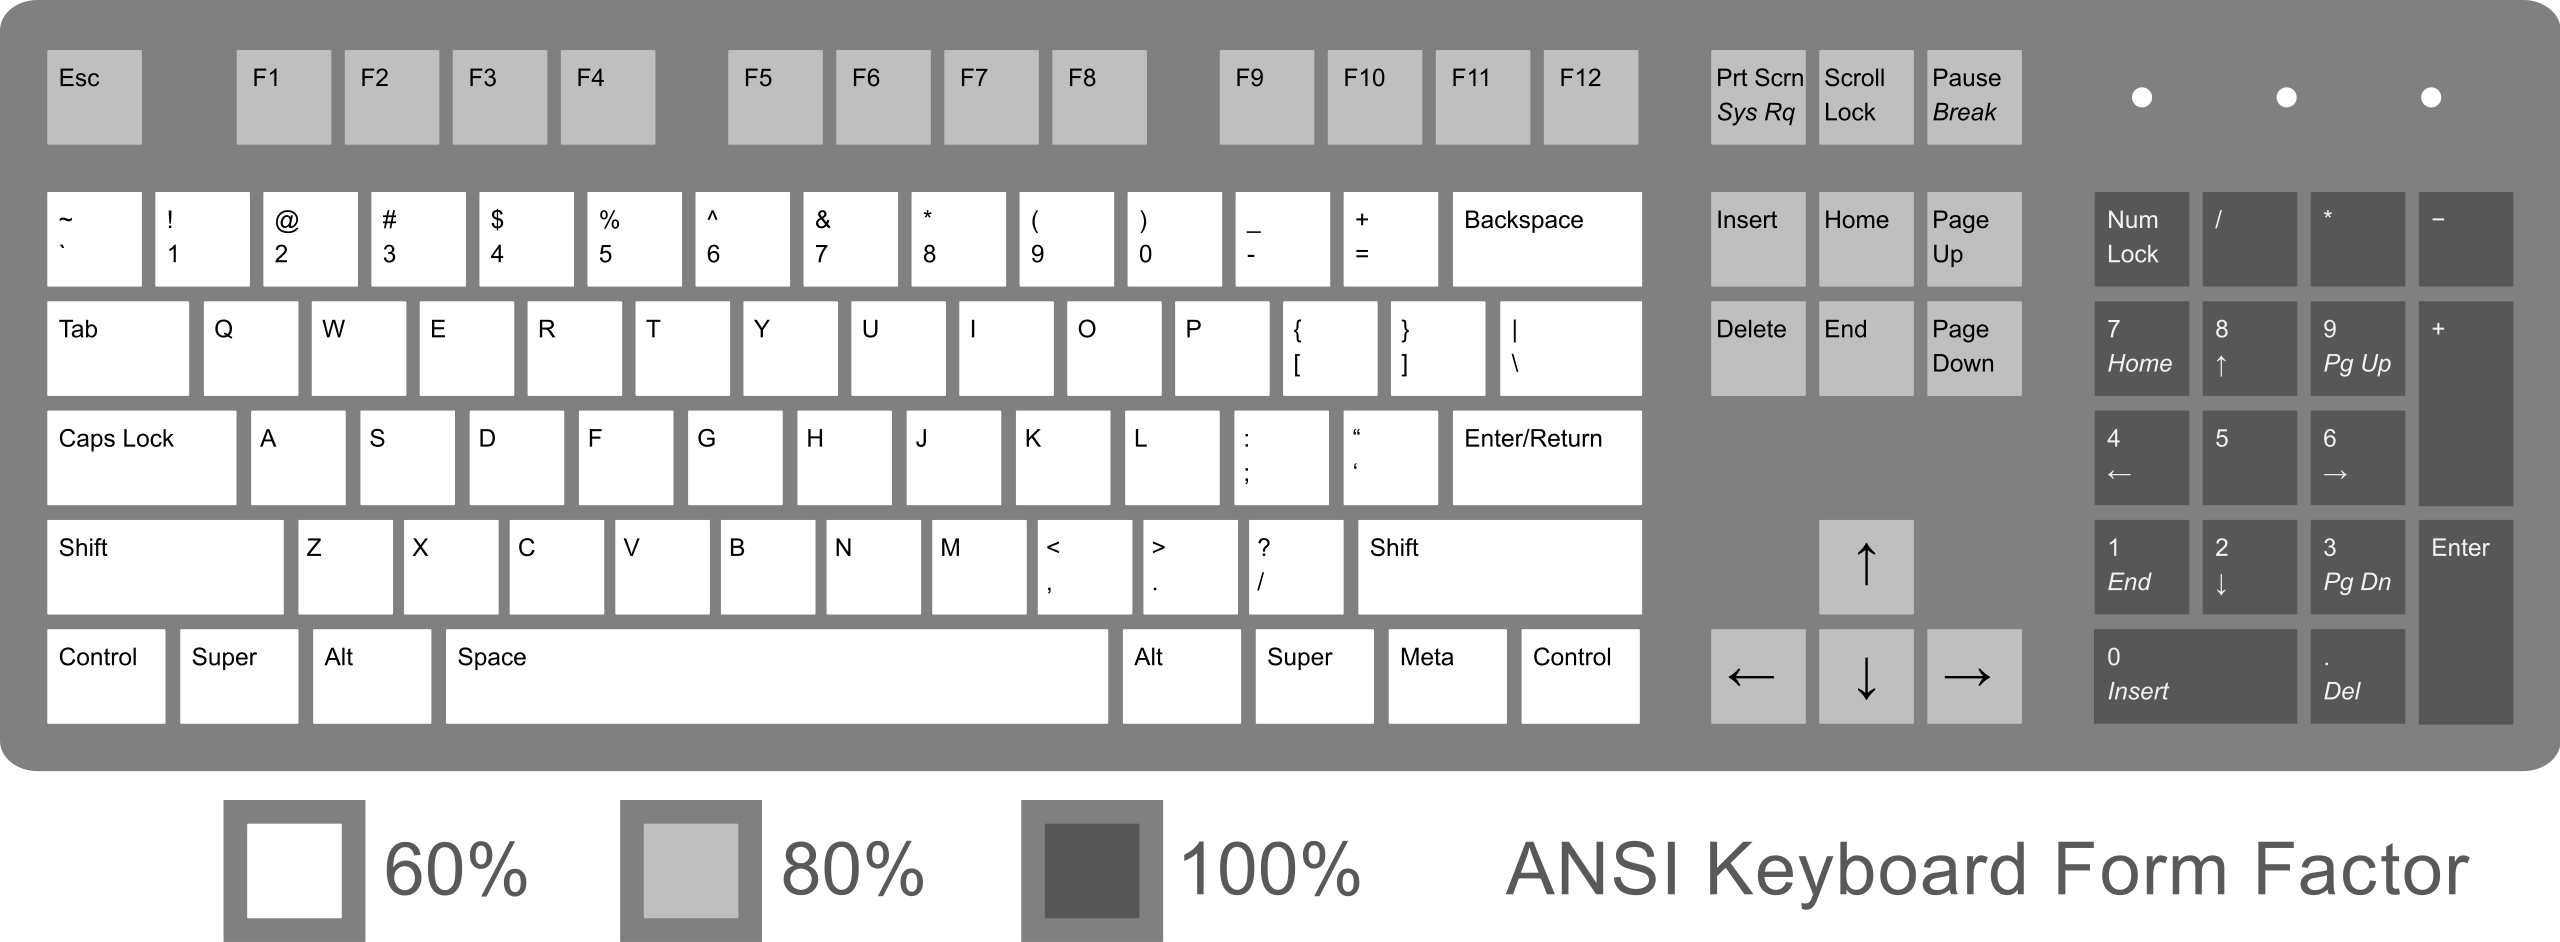
\includegraphics[width=0.8\textwidth]{ansi.png}
	\caption{\ac{ansi} Keyboard layout with form factors. Reprinted from \fullcite{figure-ansi}}
	\label{fig:ansi}
	\centering
\end{figure}

\subsubsection{Ergonomic Keyboards Layouts and Form Factors}

There have been other keyboard layouts and form factors created to mitigate
common issues associated with QWERTY layouts. These include Colemak, Dvorak, and
Alphabetical layouts. However, studies have shown that the layout itself does
not matter as beginners do not necessarily see the keyboard as a structured set,
but rather as a random collection of characters, even if it is alphabetized
\parencite{norman1982},

A different form factor has a great effect on ergonomics. One such example of a
form factor is an ergonomic keyboard developed by Microsoft called Microsoft
Natural MultiMedia Keyboard. \citeauthor{ripat2010} used this keyboard in
determining that ergonomic keyboards can help in reducing symptoms of \ac{neck}.
Figure~\ref{fig:mn} shows the layout of the Microsoft Natural MultiMedia
Keyboard.

\begin{figure}[H]
	\centering
	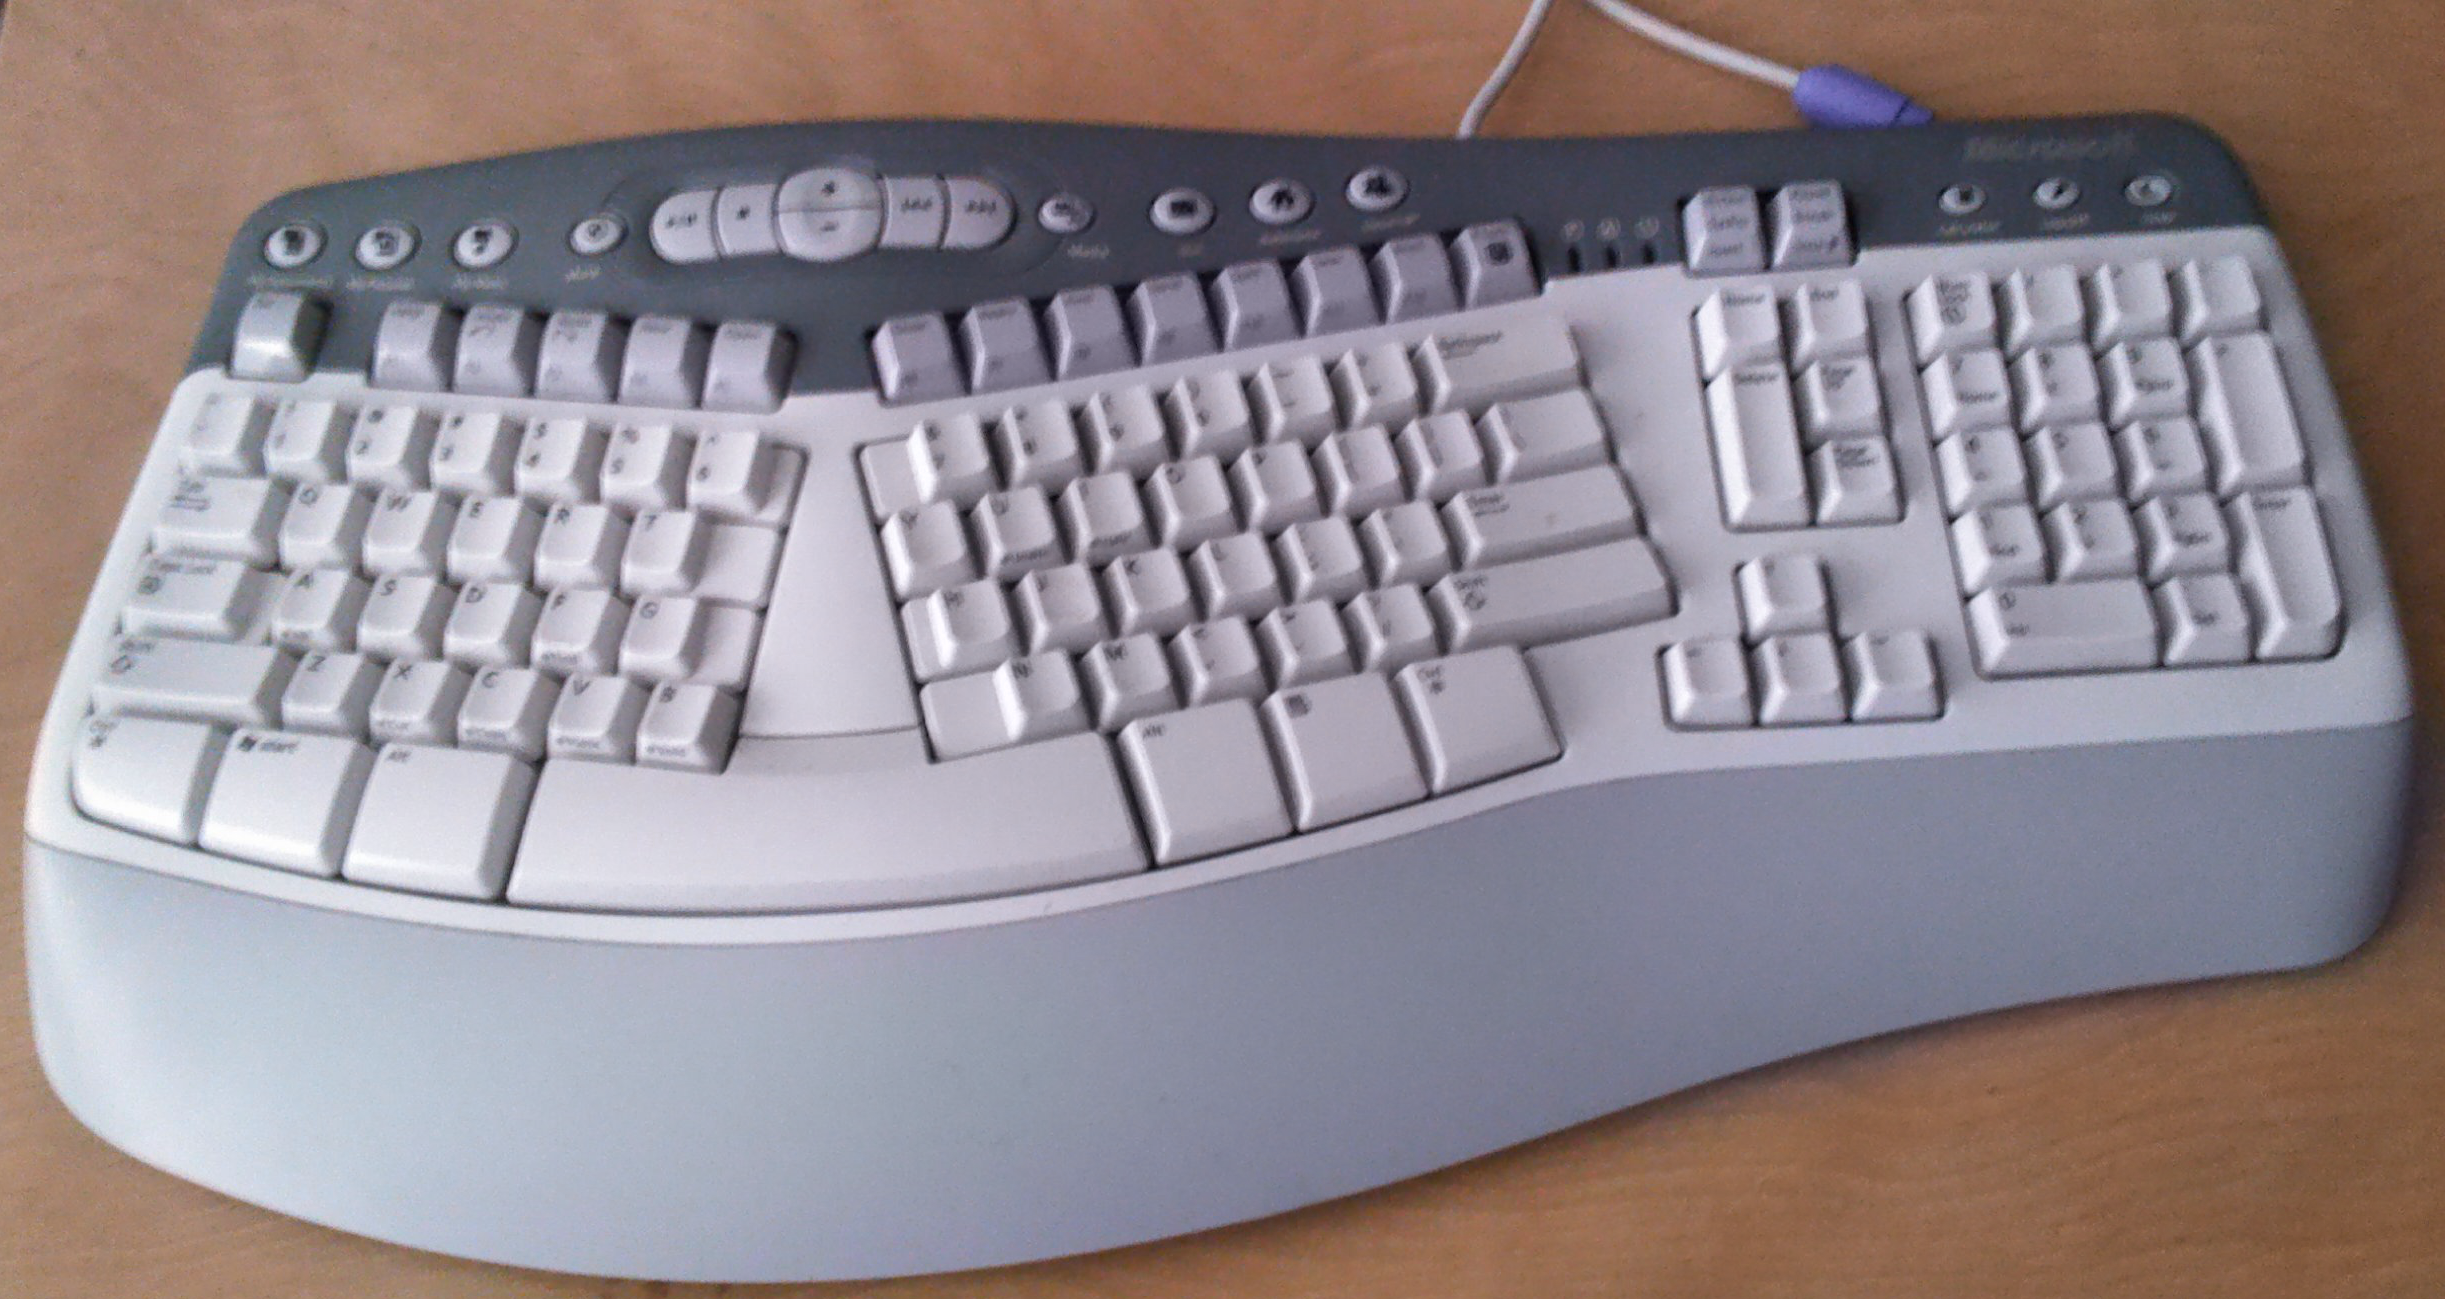
\includegraphics[width=0.8\textwidth]{mn.png}
	\caption{Microsoft Natural MultiMedia Keyboard. Reprinted from \fullcite{mn}}
	\label{fig:mn}
	\centering
\end{figure}

There are other form factors other than the full-size keyboard and variations
thereof that focus on ergonomics. One such example is a split keyboard layout
where the keyboard is split in half, one for the left hand and one for the
right. One such benefit, according to \citeauthor{ergodox}, is a more relaxed
position due to typing at shoulder width.

\subsection{Keyboard Typing Metrics}

There are numerous metrics used to quantify keyboard typing performance. Two
common metrics used in the majority of typing tests include Accuracy and Speed.

\subsubsection{Standardized Keyboard Typing Assessments}

To be able to measure these metrics, a keyboard typing assessment needs to be
done. However, there are no standardized keyboard typing assessments
\parencite{donica2018}. As such, teaching methods and assessments, like
Keyboarding without Tears, Monkeytype, and Keybr, may produce different metrics
for the same typist due to their difference in conducting the assessment.

\subsubsection{Speed}
Speed, also called as entry rate by \citeauthor{arif2009}, measures the number
of characters entered in a specific time frame. The most common metric that
measures speed is \ac{wpm}. \ac{wpm} as defined by \citeauthor{arif2009} is:

\begin{equation}
	WPM = \frac{|T| - 1}{S} \cdot 60 \cdot \frac{1}{5}
\end{equation}

where, $|T|$ is the length of the text, $S$ is the time in seconds spent writing
the text. This time starts directly after the first character has been pressed,
and ends when the last letter has been entered. As such, $1$ is subtracted from
$|T|$, as the time spent to find and press the first character cannot be
accurately determined. However, some typing assessments do not subtract $1$ from
$|T|$. $60$ refers to the number of seconds in a minute and $\frac{1}{5}$
normalizes the metric for the average length of words.


Other metrics also measure speed but they aren't as commonly used as \ac{wpm}.
These include Characters per Minute, Gestures per Second, Adjusted Words per
Minute, and Keystrokes per Second

\subsubsection{Accuracy}
Accuracy measures the number of correctly pressed characters in an input string.
Accuracy, as defined by \citeauthor{bartnik2021}, is:

\begin{equation}
	ACC = \frac{|C|}{|T|} \cdot 100\%
\end{equation}

where $|C|$ is the number of correct characters and $|T|$ is the length of the
text.

The inverse of accuracy is error rate, where the number of incorrectly pressed
characters is measured instead. \citeauthor{arif2009} describe 5 common error
rate metrics: Error Rate, Minimum String Distance Error Rate, Keystroke per
Character, Erroneous Keystroke Error Rate, and Total Error Rate.

\subsubsection{Limitations of the Metrics}
These metrics are all based on the inputted characters by the user. These
metrics do not take into account other aspects of keyboard typing such as
posture, hand and wrist positions, and finger placement. Consequently, these
metrics do not give a full picture of the performance of the person typing and
they only provide a cursory view of how a person types.

\subsection{Keyboard Typing Methodology}
Keyboard typing can be accomplished in numerous ways. The main difference
between the different methodologies is the number of fingers used when typing
and how the typist navigates the keyboard to find the keys. The methodology
ranges from Hunt and Peck to Touch Typing, with variations of the two in
between.

Hunt and Peck uses one finger on one hand to press a key. This method is aided
by using vision to locate the specific key to press \parencite{hoot1986}. On the
other hand, Touch typing uses standard QWERTY mapping to type without using
visual cues. \parencite{dobson2009touch} This mapping involves assigning certain
fingers to certain keys. Figure~\ref{fig:touch-type} is the standard QWERTY
mapping used for an \ac{ansi} layout. Kinesthesis and proprioception are used in
locating the keys \parencite{logan2016}.

\begin{figure}[H]
	\centering
	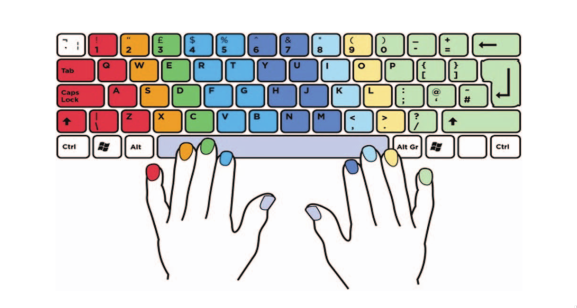
\includegraphics[width=0.8\textwidth]{touch-type.png}
	\caption{Standard QWERTY mapping for \ac{ansi}. Reprinted from \fullcite{logan2016}}
	\label{fig:touch-type}
	\centering
\end{figure}


\section{Keyboard Typing in Education}

Today, students are expected to type essays, articles, and other submissions
using word processors \parencite{poole2016}. Testing is also commonly done using
computerized assessments which require the need for keyboards
\parencite{moodle}. As such, there is a need for students to be well versed in
keyboard typing and for keyboard typing to be part of the curriculum.

Keyboard typing has been a part of this curriculum for a long time, with studies
about effective methods to teach keyboard typing reaching as far back as 1986
\parencite{hoot1986}. Studies have continued to this day to continue to optimize
and improve methods of teaching keyboard typing to students.

These studies start teaching kids in the kindergarten level and the studies try
to optimize the teaching methods to improve the speed and accuracy of typing of
the learners. By starting to teach touch typing to students early, these
students will develop the potential for higher-level keyboard typing
\parencite{donica2018}.

\subsection{Expectations of Keyboard Proficiency}

In the United States, keyboard typing is an expected learning outcome for third
grade in the Common Core State Standards \parencite{ccs}. At this grade level,
only basic keyboard typing skills are required. By fourth grade, students are
expected to have enough proficiency to type one page in one sitting. This is
increased to two pages by fifth grade.

In the Philippine context, the \citeauthor{deped} expects learners with a mental
age of 4--6.9 years old to use correct posture and locate characters, learners
with a mental age of 7--11.9 are introduced to home row finger placement, and
learners with a mental age of 12 and above are expected to ``use proper typing
technique with efficiency and accuracy without looking at the keyboard''
\parencite{deped}.

\subsection{Current Teaching Methods}

Current teaching methods involve replicating a given text. Learners then copy
the text into a given text field that records the typed characters. Correct and
incorrect characters are then identified, and suitable errors are presented.
Afterward, metrics, such as \ac{wpm}, and accuracy are given
\parencite{bartnik2021, typeracer}.

Through this process, the learner goes through the three stages of Motor
Learning Theory. The student undergoes the cognitive stage where they try to
understand and create strategies to accomplish the given task. Then the
associative stage follows where the strategies and skills learned from the
previous stage are refined. At this stage, the learners are expected to rely less
on visuals to locate the keys and more on kinesthesis. By the final stage, the
autonomous stage, the learner does not rely on visuals at all and focuses on
using kinesthetic feedback to find the keys. By this point, the learner has
progressed from using Hunt and Peck, to becoming proficient in touch typing.
\parencite{donica2018}

\subsubsection{Keyboarding without Tears}

Keyboarding without Tears is a web-based application and curriculum that teaches
students touch typing. However, one key differentiator of this curriculum is the
usage of a row-based standard mapping, rather than a column-based standard
mapping that is common in other teaching guides. Figure~\ref{fig:kwt} shows the
standard mapping used in this curriculum.

This curriculum is self-directed and learners can learn at their own pace. At
its core, the curriculum is designed to be 36-week long with 5-10 minutes of
lessons per day. The lessons in the curriculum follow the three stages of
Motor Learning Theory \parencite{kwt}.

\begin{figure}[H]
	\centering
	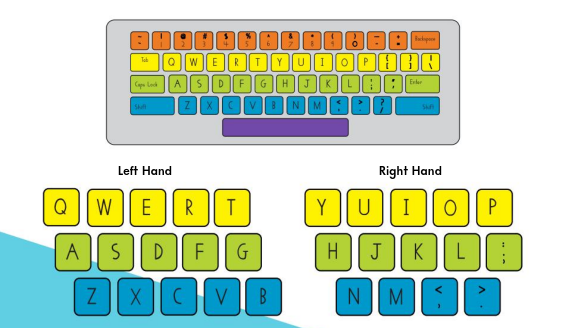
\includegraphics[width=0.8\textwidth]{kwt.png}
	\caption{Row based standard mapping. Reprinted from \fullcite{kwt}}
	\label{fig:kwt}
	\centering
\end{figure}


\subsubsection{Monkeytype, Typeracer}

These two keyboard typing tests are similar. They follow a common experience
where users type a predetermined phrase, quote, or random words, and metrics are
given after the test. Afterward, the learners may try the test again, or choose
another set of words to type. These typing tests do not have a structured
curriculum for learning how to touch type. It is left to the learner to practice
and learn on their own \parencite{bartnik2021, typeracer}.

\subsubsection{Keybr}

Keybr is similar to Monkeytype and Typerace, in that they also have the users
type a predetermined phrase, quote, or random words. However, this application
has more guidance compared to the two. Keybr uses statistics to create typing
lessons that are appropriate to the current typing proficiency of the learner.
The words selected are random at first, and the skill level of the learner is
determined by the performance of the user with these words and characters. The
information gathered is then used to generate new words for the next iteration.
As an example, if a learner has difficulty in typing the letter q, the next
iterations will have a lot of words that contain the letter q.

Statistics from their website show that this learning method is successful, with
some learners improving their typing speed by 20--40 \ac{wpm} \parencite{keybr}.

\section{Keyboard Typing in Health}

There have been a lot of studies that show the effect of keyboard typing, and
its associated movements (or lack thereof), has an effect on the human body.
These studies have shown that keyboard typing has an effect on our neck, shoulder,
upper limb, wrist, arms, and fingers \parencite{szeto2005, baker2007digit}

\subsection{Health Issues arising from Keyboard Typing}

\ac{neck} are a common issue that is associated with an elongated length of time
maintaining a static posture. When using the computer, the posture commonly
adapted by users has the neck and shoulder regions in a static hold for a long
time. This results in forward neck flexion and increased muscle tension
\parencite{szeto2005}.

In addition, it has been shown that 22\% of computer users sustain
musculoskeletal disorders of the upper extremity. This includes the neck,
shoulder, hands, and wrists. \parencite{gerr2002}

Carpal tunnel syndrome is also a common issue in the general population. This is
caused by the chronic compression of the median nerve. There is a common belief
that typing is one main cause for the disorder \parencite{carpal-myth}. There
are no definite conclusions if this myth is true, however, a study by
\citeauthor{toosi2015} found that typing causes ulnar deviation, especially if
done without proper form. This ulnar deviation contributes to the swelling of
the median nerve during and after typing. However, the authors noted that it is
unclear if this swelling leads to long-term nerve injury.

\subsection{Finger and Wrist Kinematics}
The way people move their hands, wrists, and fingers differ between each person.
This can be attributed to the different typing styles each person has. One key
difference between people is the angle of the 5th digit.

However, there are some common movements and positions regardless of typing
style: flexion, or the curving of the fingers, across the fingers, is decreasing
across the hand, with the 2nd digit having the least flexion. This may be due to
the instinct to reduce pronation of the hand, which in turn increases the
distance of the 2nd digit to the keyboard. In addition, some people isolate or
extend one of their thumbs, usually the one not used for pressing a key. This is
also true for some people that do not use their 5th digit during typing
\parencite{baker2007}.

The movement and angle of the wrists also depend on the typing style of the
typists. Some people do not reposition their hands, while others do. This
difference comes from the way these people reach for certain far-away keys. Some
stretch their fingers to reach far-away keys, while others move their entire
hand to reach these keys.

For those that reach their keys by stretching their fingers, there is an
increased probability that the wrists and fingers adapt non-neutral postures.
These include wrist extension, ulnar deviation, and pronation, which may cause
musculoskeletal disorders of the upper extremity (\cite{marklin1999} as cited in
\cite{baker2007})

\section{Finger and Hand Tracking}
Finger and Hand tracking is a method of tracking fingers and hands in 3D space
using motion capture systems or computer vision. This technique allows computers
to perform actions and analyses on the motions and positions of these body
parts.


\subsection{Types of Tracking}

\subsubsection{Hardware Aided Solutions}

Motion Capture Systems allow for capturing detailed skeletal motion in humans.
These systems usually capture full-body motion, focusing on large parts of the
human body, such as the torso, limbs, and head.

However, motion capture systems have difficulty in tracking more articulated
body parts --- with the fingers being one of them. The industry standard for
capturing finger movements is through the use of an optical marker-based motion
capture system. This is due to its ability to capture natural motion accurately.

This method uses cameras to triangulate the 3D location of markers attached to
the limbs of a person. For finger tracking, 13--20 markers are placed on the
fingers, and cameras are brought closer to track the small movements of the
finger \parencite{wheatland2015}.

But this method is cost-prohibitive, and cannot handle occlusions well.
\citeauthor{alexanderson2016} present a method for an optical marker-based
motion capture system that can predictably recover from self-occlusion and has a
better performance compared to previously used algorithms, however, the issue of
cost and self-occlusion still persists.

Bend-sensor gloves are also an option for finger tracking. These gloves have
sensors within them that track joint angles in the hand and fingers. One key
differentiator of this solution compared to the others is the removal of
self-occlusion in the data. As such, this is commonly used in sign language, and
gesture recognition due to its accuracy.

However, these gloves need a lot of time to calibrate as cross-coupling of the
sensors proves a problem. Cross-coupling is prevalent because the movement of
one finger also moves other parts of the hand. These movements may cause a
sensor aimed to track a specific movement of a different part of the hand to
inadvertently detect a movement when there should be none
\parencite{wheatland2015}.

\subsubsection{Computer Vision}

At its core, Computer Vision aims to perform tasks that the human visual system
can do \parencite{cern}. This includes object classification, tracking, and
gesture recognition, and face recognition. At the present, most computer vision
systems utilize deep learning algorithms, and convolutional networks to gather
information from an image, or a set of images. One such example of a
convolutional network used in computer vision is Inception by
\citeauthor{szegedy2015} which proposes a convolutional neural network
architecture for object classification and detection.

\subsection{Available CV Solutions for Tracking}

\subsubsection{OpenCV}

OpenCV is an open-source computer vision and machine learning software library
that houses ${\approx2500}$ optimized algorithms. This library is widely used by
companies, researchers, and open source communities that utilize computer vision
and machine learning in their projects. Examples of companies that use OpenCV
include Google, Sony, and Honda.

The library has C++, Python, Java, and Matlab interfaces. The library also supports
Windows, Linux, Android, and macOS, allowing for great developer experience, and
wide deployment capabilities \parencite{opencv}.

\subsubsection{MediaPipe}
\label{section:rrl-mediapipe}

MediaPipe is an open-source computer vision framework that allows developers to
create a perception pipeline. This perception pipeline is a directed graph of
calculators. Data passes through the graph as packets and a group of packets
constitute a data stream. As the data passes through the pipeline, the
calculators, produce the desired output.

This framework allows for performant object detection, hand and finger tracking,
human pose detection. The framework also allows for combining multiple features,
by adding them to the graph as calculators. MediaPipe has C++, Python, JS, and
Coral interfaces. It also supports Android and iOS devices
\parencite{mediapipe}.

\subsubsection{MATLAB}
MATLAB is a programming platform for the analysis and designing of systems.
MATLAB is commonly used by engineers and scientists for computational
mathematics \parencite{what-matlab}.

A toolbox offered by MATLAB is the Computer Vision Toolbox that contains
algorithms, and functions for use in the development of computer vision, 3D
vision, and video processing systems. By using the available algorithms in the
toolbox, such as YOLOv2, and ACF, hand detection and gesture recognition is made
possible in the platform \parencite{matlab}.

\subsection{Applications}

There have been multiple applications and products that utilize hand and finger
tracking as their main component.

\cite{dorf2001} presents a use case for finger tracking in augmented
environments. In the paper, interaction in a virtual environment through the use
of gestures. The tracking system uses an optical marker-based motion capture
system where the user wears a glove with retroreflective markers.

\cite{chiang2014} used a Kinect, a 3D sensing device by Microsoft that
uses depth data, to track fingers to play virtual instruments. Virtual Pianos
and Guitars were created and played with reliable and stable tracking.

\cite{yousaf2014} created a virtual keyboard that operates using finger
tracking. The tracking uses the movement of the finger joints as the basis for
selecting which key to press. A camera captures the movement, and the resulting
video stream is used for hand region detection and finger joint localization.
Using probabilistic regional density-based kernel tracking, finger joint
trajectories are gathered. Feature vectors are then interpreted from the
trajectories. These feature vectors are used in logic-based techniques and
Dynamic Bayesian Network for classification, detection, and recognition of
keystrokes.

\section{Summary of the Research Gap}
While there are a lot of applications and curriculum aimed at teaching touch
typing, there is no automated system available that detects if a person uses the
correct finger to press a key.

By having this system, educators can accurately determine if and when a student
is having a hard time typing and if these students will need an intervention to
correct mistakes.

This is also important because certain movements and hand positions will cause
nerve and muscular disorders that will impact the user. By correcting these
problematic movements and hand positions, these disorders can be prevented.

\chapter{Methodology}

\section{Setup}
\label{section:metho-setup}

The experimental setup and configuration will be composed of three elements: the
camera, the keyboard, and the environment. Figure~\ref{fig:metho-setup-cam}
shows the sketch of the complete experimental setup.

\begin{figure}[H]
	\centering
	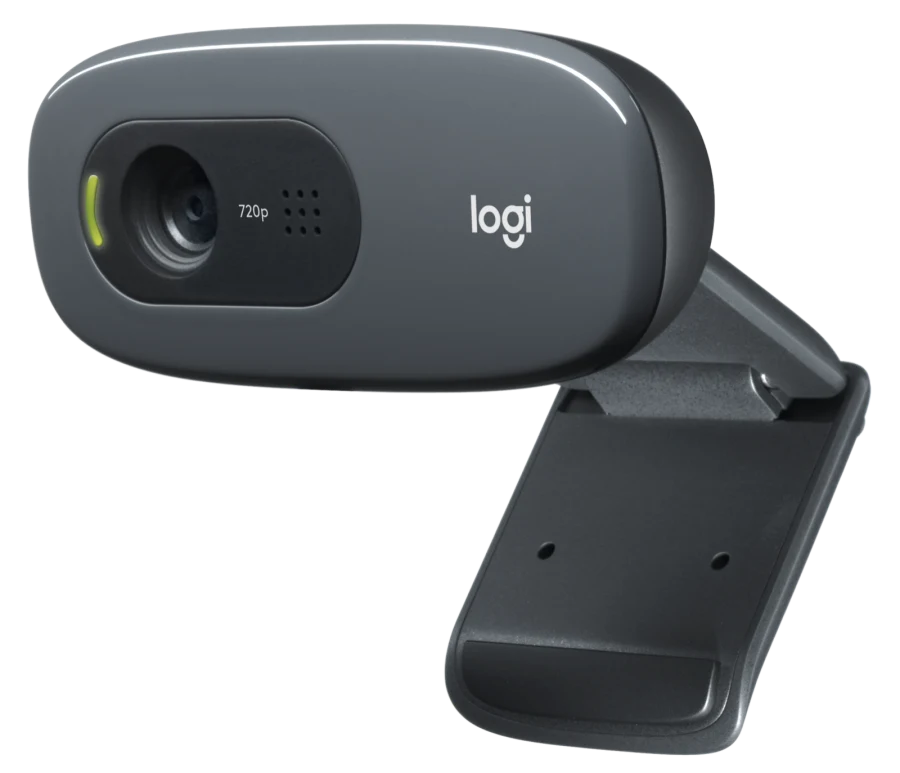
\includegraphics[width=0.4\textwidth]{webcam.png}
	\caption{Sketch of the experimental setup}
	\label{fig:metho-setup-cam}
	\centering
\end{figure}

\subsection{Camera}
The camera setup will use a single monocular camera positioned in a top-down
view. The camera will capture the entirety of the keyboard and the movement of
the ten fingers. To do so, it will be mounted on top of the monitor and the
camera will point down towards the table. Figure~\ref{fig:metho-setup-keeb}
illustrates what the camera will capture once placed in its correct position.

\begin{figure}[H]
	\centering
	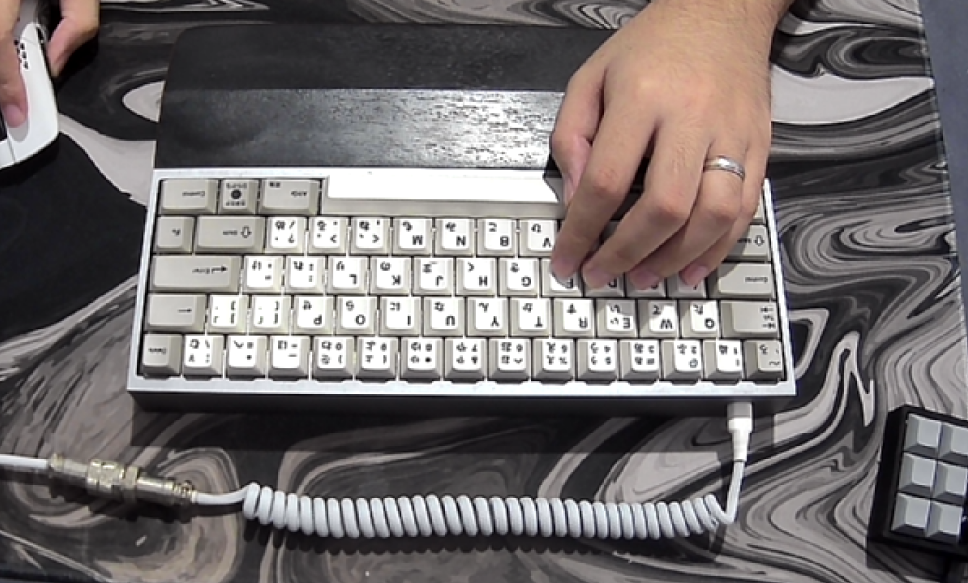
\includegraphics[width=0.8\textwidth]{actual-keeb.png}
	\caption{Keyboard, camera angle, and placement to be used for testing.}
	\label{fig:metho-setup-keeb}
\end{figure}

The specific camera to be used will be a Logitech C920.
Figure~\ref{fig:metho-setup-cam} is a picture of this camera. It is a 3 mega pixel
webcam that is capable of capturing color video in 1080p/30fps and 720p/30fps
with a diagonal field of view of 78\degree. This camera has a universal mounting
clip that will allow the camera to be correctly positioned within the
experimental setup \parencite{logitech}.

\begin{figure}[H]
	\centering
	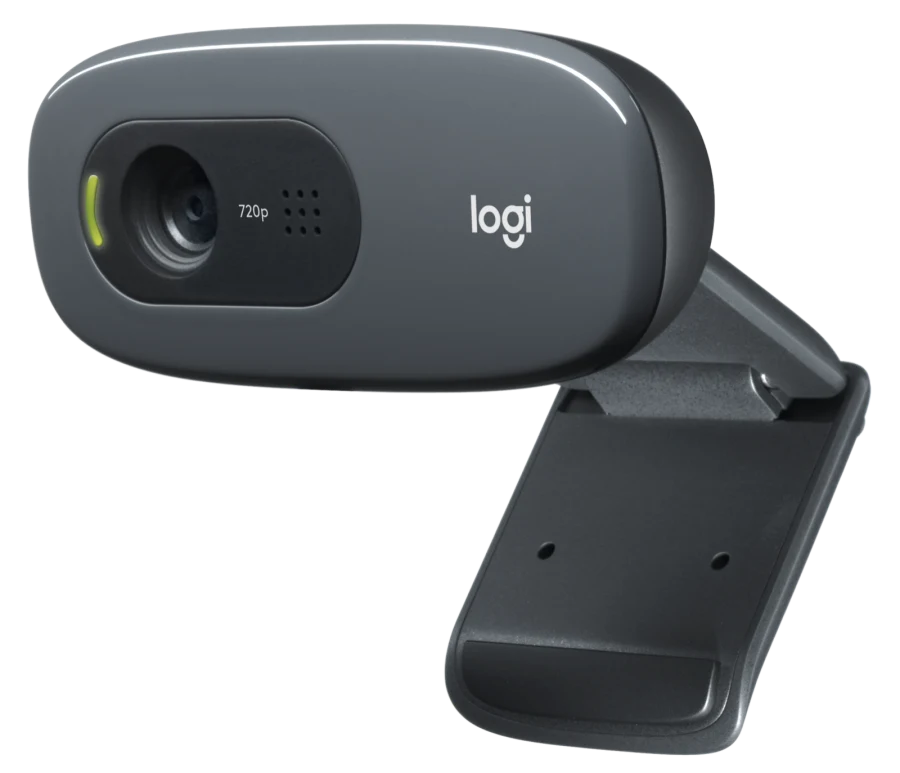
\includegraphics[width=0.4\textwidth]{webcam.png}
	\caption{Logitech C920. Reprinted from \fullcite{logitech}}
	\label{fig:metho-setup-cam}
	\centering
\end{figure}

\subsection{Keyboard}
\label{section:metho-keeb}

The keyboard will be a 60\% keyboard as shown in
Figure~\ref{fig:metho-setup-keeb}. This will limit the necessary mapping for the
algorithm to the alphanumeric portion of the keyboard. This keyboard choice will
also lessen the area that the camera will need to capture, as this keyboard type
is considerably smaller compared to a full-size keyboard. The keyboard will have
key caps and a case in a light color that will contrast the dark surface that it
will be placed on. This is to improve initial keyboard detection. In addition,
the keyboard layout will also be ANSI, due to the availability and widespread
adoption of the layout in the Philippines.

\subsection{Environment}
The environment the setup would be placed in would be a well lit environment
with a light source beside the camera. This light source will evenly light the
keyboard and the fingers used for typing. The light source to be used will be a
common LED desk lamp rated at 9 Watts with 700 lumens. This light will be white
with a color temperature of 6500k.

In addition, the surface where the keyboard is to be placed on will be solid
green without any variation of color. This is to improve initial keyboard
detection.

\section{Algorithm}
\label{section:metho-algo}

\subsection{Computer Vision based Keyboard Detection, and Mapping}
\label{section:metho-algo-keyboard}

A computer vision algorithm will be created as a starting point for detecting,
and mapping the keyboard within a video. The flowchart of the algorithm is shown
in Figure~\ref{fig:metho-algo-key-flow}.

\begin{figure}[H]
	\centering
	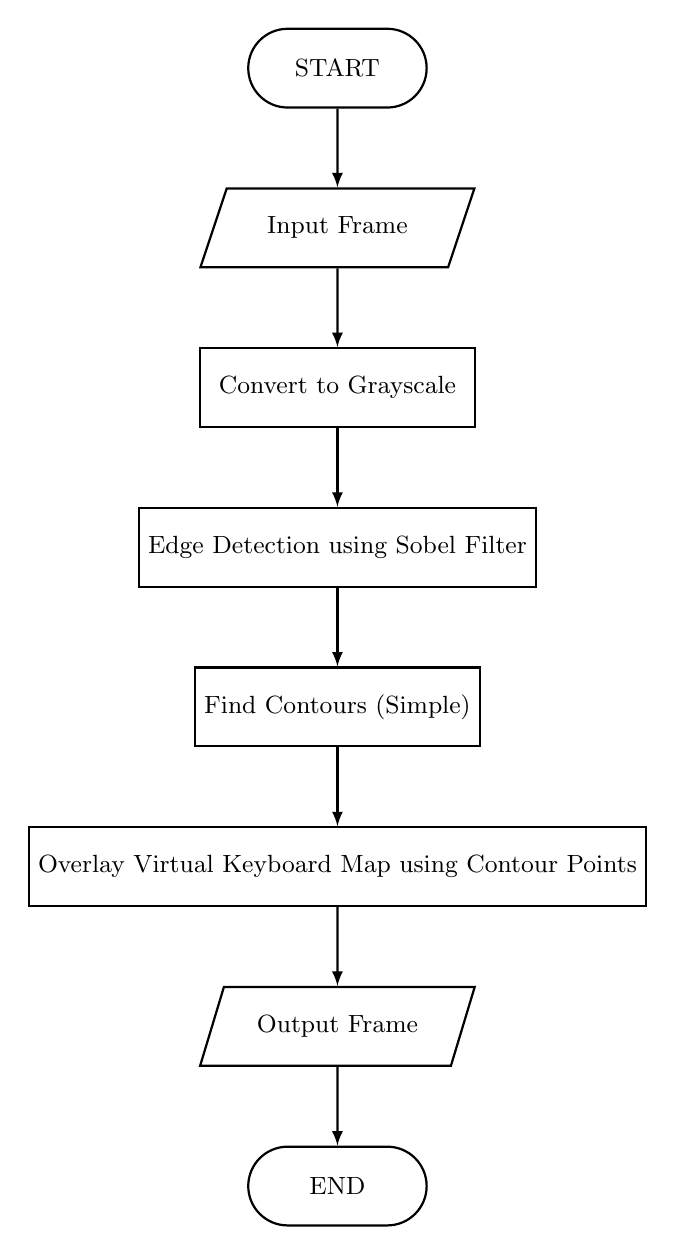
\begin{tikzpicture}[font=\small,thick]
		\node[draw,
			rounded rectangle,
			minimum width=2.5cm,
			minimum height=1cm] (start) {START};

		\node[draw,
			trapezium,
			trapezium left angle = 65,
			trapezium right angle = 115,
			trapezium stretches,
			below=of start,
			minimum width=3.5cm,
			minimum height=1cm
		] (input) {Input Frame};

		\node[draw,
			below=of input,
			minimum width=3.5cm,
			minimum height=1cm] (gray) {Convert to Grayscale};

		\node[draw,
			below=of gray,
			minimum width=3.5cm,
			minimum height=1cm] (sobel) {Edge Detection using Sobel Filter};

		\node[draw,
			below=of sobel,
			minimum width=3.5cm,
			minimum height=1cm] (contours) {Find Contours (Simple)};

		\node[draw,
			below=of contours,
			minimum width=3.5cm,
			minimum height=1cm] (map) {Overlay Virtual Keyboard Map using Contour Points};

		\node[draw,
			trapezium,
			trapezium left angle = 65,
			trapezium right angle = 115,
			trapezium stretches,
			below=of map,
			minimum width=3.5cm,
			minimum height=1cm
		] (output) {Output Frame};

		\node[draw,
			below=of output,
			rounded rectangle,
			minimum width=2.5cm,
			minimum height=1cm] (end) {END};

		\draw[-latex] (start) edge (input)
		(input) edge (gray)
		(gray) edge (sobel)
		(sobel) edge (contours)
		(contours) edge (map)
		(map) edge (output)
		(output) edge (end);

	\end{tikzpicture}
	\caption{Flowchart of Keyboard Detection and Mapping Algorithm}
	\label{fig:metho-algo-key-flow}
\end{figure}

\subsubsection{Convert to Grayscale}
The frame will be converted to a 256 level grayscale image. This step will be
performed because future steps of the algorithm will not require color values to
work. In addition, the performance of the following steps will be also improved
as the number of dimensions to be analyzed is reduced.

\subsubsection{Edge Detection using Sobel Filter}
A Sobel Filter is an edge detection filter that uses a 3$\times$3 kernel that is
convolved twice. Once horizontally, and another vertically to produce a
grayscale image of the outlines within the frame. The kernels used by the Sobel
Filter \parencite{sobel2014} is shown in Figure~\ref{fig:metho-algo-key-sobel}.

\begin{figure}[H]
	\centering
  $\begin{bmatrix}
  +1 & 0 & -1\\
  +2 & 0 & -2\\
  +1 & 0 & -1
  \end{bmatrix}$
	and
  $\begin{bmatrix}
  +1 & +2 & +1\\
  0 & 0 & 0\\
  -1 & -2 & -1
  \end{bmatrix}$
	\caption{Sobel Operator Kernels. Reproduced from \fullcite{sobel2014}}
	\label{fig:metho-algo-key-sobel}
\end{figure}

The expected result of this step is a black and white image that highlights the
edges of the keyboard in white.

\subsubsection{Find Contours (Simple)}
\label{section:metho-algo-key-contours}
Contours are curves joining all continuous points that have the same color or
intensity \parencite{opencv-contours}. In this algorithm the OpenCV function
\texttt{findContours} will be used to find the contours of the outlines of the
object found using the previous step. This function accepts a contour
approximation method as one of its arguments. Two methods are provided by
OpenCV, \texttt{CHAIN\_APPROX\_NONE} and \texttt{CHAIN\_APPORX\_SIMPLE}. The
former returns all contours in the shape, while the latter removes redundant
points and returns the least amount of points that describes the shape. The
algorithm will use the latter, as only the extreme edges of the keyboard needs
to be detected. This OpenCV function implements the algorithm of
\cite{contours} in their paper ``\citefield{contours}{title}''.

The expected result of this algorithm is four contour points which are
positioned on the four edges of the keyboard.

\subsubsection{Overlay Virtual Keyboard Map using Contour Points}
The virtual keyboard map is a rectangular image that contains individual region
of interest (ROI) for each key in a 60\% \ac{ansi} keyboard. Each key has a
corresponding color assigned to it and this color fills the region where this
key is located at. Figure~\ref{fig:metho-algo-key-map} is the virtual keyboard
map.

\begin{figure}[H]
	\centering
	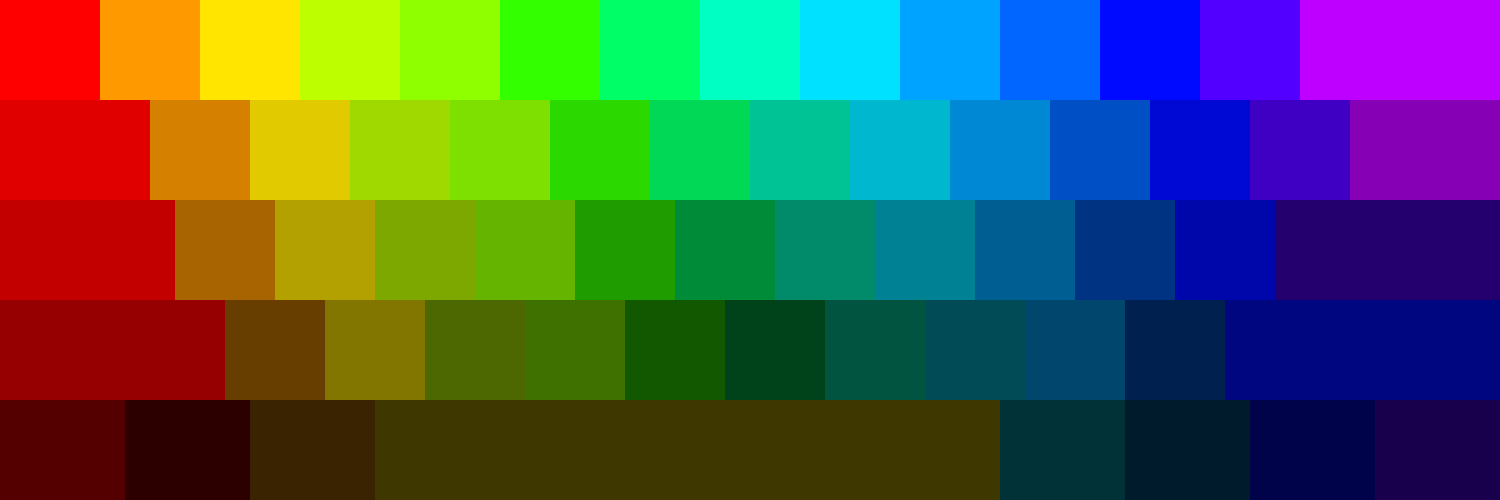
\includegraphics[width=0.6\textwidth]{image-map.png}
	\caption{Initial Image Map}
	\label{fig:metho-algo-key-map}
	\centering
\end{figure}

The virtual map will then be stretched over the object, with the four contour
points as the four edges of the virtual keyboard map. The image generated will
then be returned as the final output of the graph.
Figure~\ref{fig:metho-algo-key-overlay} illustrates this image, and
Figure~\ref{fig:metho-algo-key-half} shows how accurate the image map is when
overlaid over the image.

\begin{figure}[H]
	\centering
	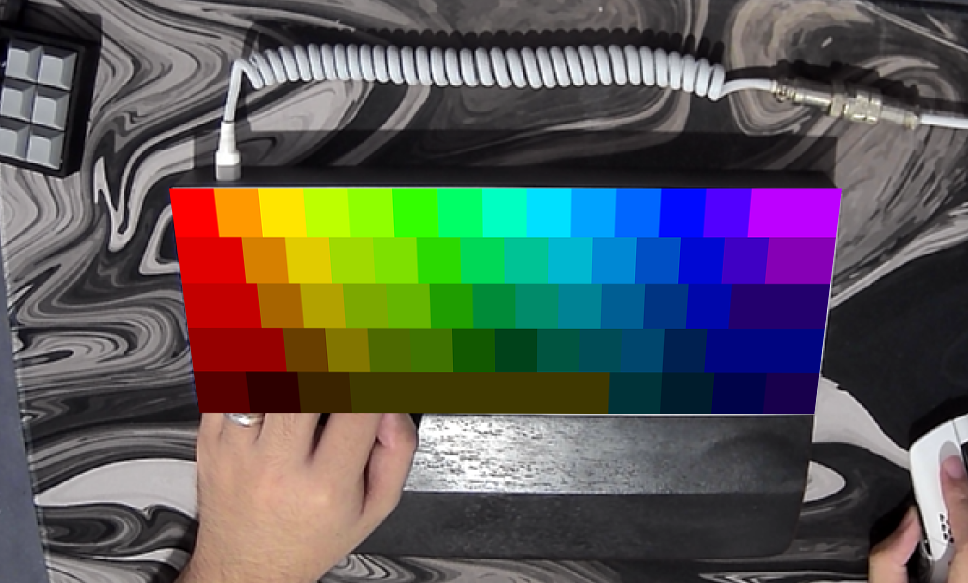
\includegraphics[width=1\textwidth]{image-map-final.png}
	\caption{Expected output of the algorithm}
	\label{fig:metho-algo-key-overlay}
	\centering
\end{figure}

\hfill

\begin{figure}[H]
	\centering
	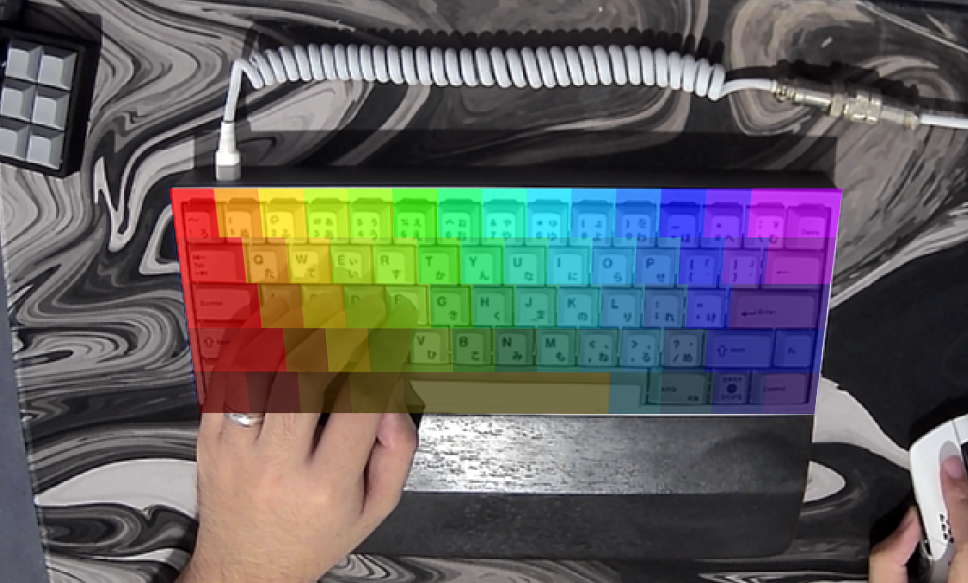
\includegraphics[width=1\textwidth]{image-map-half.png}
	\caption{Overlaid image map shown at 60\% opacity}
	\label{fig:metho-algo-key-half}
	\centering
\end{figure}

\subsection{Computer Vision based Finger Detection, and Tracking}
\label{section:metho-algo-finger}
A computer vision algorithm will be chosen as a starting point for detecting,
and tracking fingers within a video. The specific algorithm used for finger
detection and tracking will be the solution offered by MediaPipe dubbed
MediaPipe Hands. This algorithm is composed of two ML models working in
conjunction to be able to detect the different parts of the hands and track them
accurately.

\subsubsection{Palm Detection Model}
The first model, the Palm Detection Model detects the initial hand locations
using a single shot detector model based on the paper by \cite{ssd}. This model
achieves an average precision of 95.7\% in palm detection
\parencite{mediapipe-hands}.

MediaPipe Hands detects the palms first, instead of the whole hands with one
model because the hands lack high contrast patterns. This reduces the model's
ability to detect the hand with accuracy. In addition, detecting a palm is
simpler compared to detecting hands with articulated fingers since estimating a
bounding box around a rigid objects, i.e.\ a palm, is much simpler. Furthermore,
a palm can be modeled using only square anchors reducing the number of anchors
by a factor of 3--5 \parencite{mediapipe-hands}.

\subsubsection{Hand Landmark Model}
After the palms have been detected and an appropriate anchor has been
established, the Hand Landmark Model pinpoints 21 3D hand-knuckle coordinates
inside the detected hand. This is done using direct coordinate prediction.

This model was trained using 30,000 manually annotated, real-world images with
21 3D hand-knuckle coordinates. Using this information, the model can also
accurately add landmarks to partially visible hands and hands with
self-occlusion. This is also made possible by the model's consistent internal
hand pose representation \parencite{mediapipe-hands}.

\subsection{Integration for finger-key identification and mapping}

The two previously chosen algorithms will be combined to accomplish finger-key
identification and mapping. Finger-key identification refers to identifying
which finger is used to press which key. As an example, the key Q was pressed
with the pinky finger of the left hand.

The integration of the algorithm is a two step process. The first step is to get
the mapping of the keyboard using the algorithm shown in
Section~\ref{section:metho-algo-keyboard}.

The second step is a continuous loop where the mapping of the keyboard is used
in conjunction with the finger tracking algorithm chosen in
Section~\ref{section:metho-algo-finger}. The flowchart of the algorithm is shown
in Figure~\ref{fig:metho-algo-integration}

\begin{figure}[H]
	\centering
	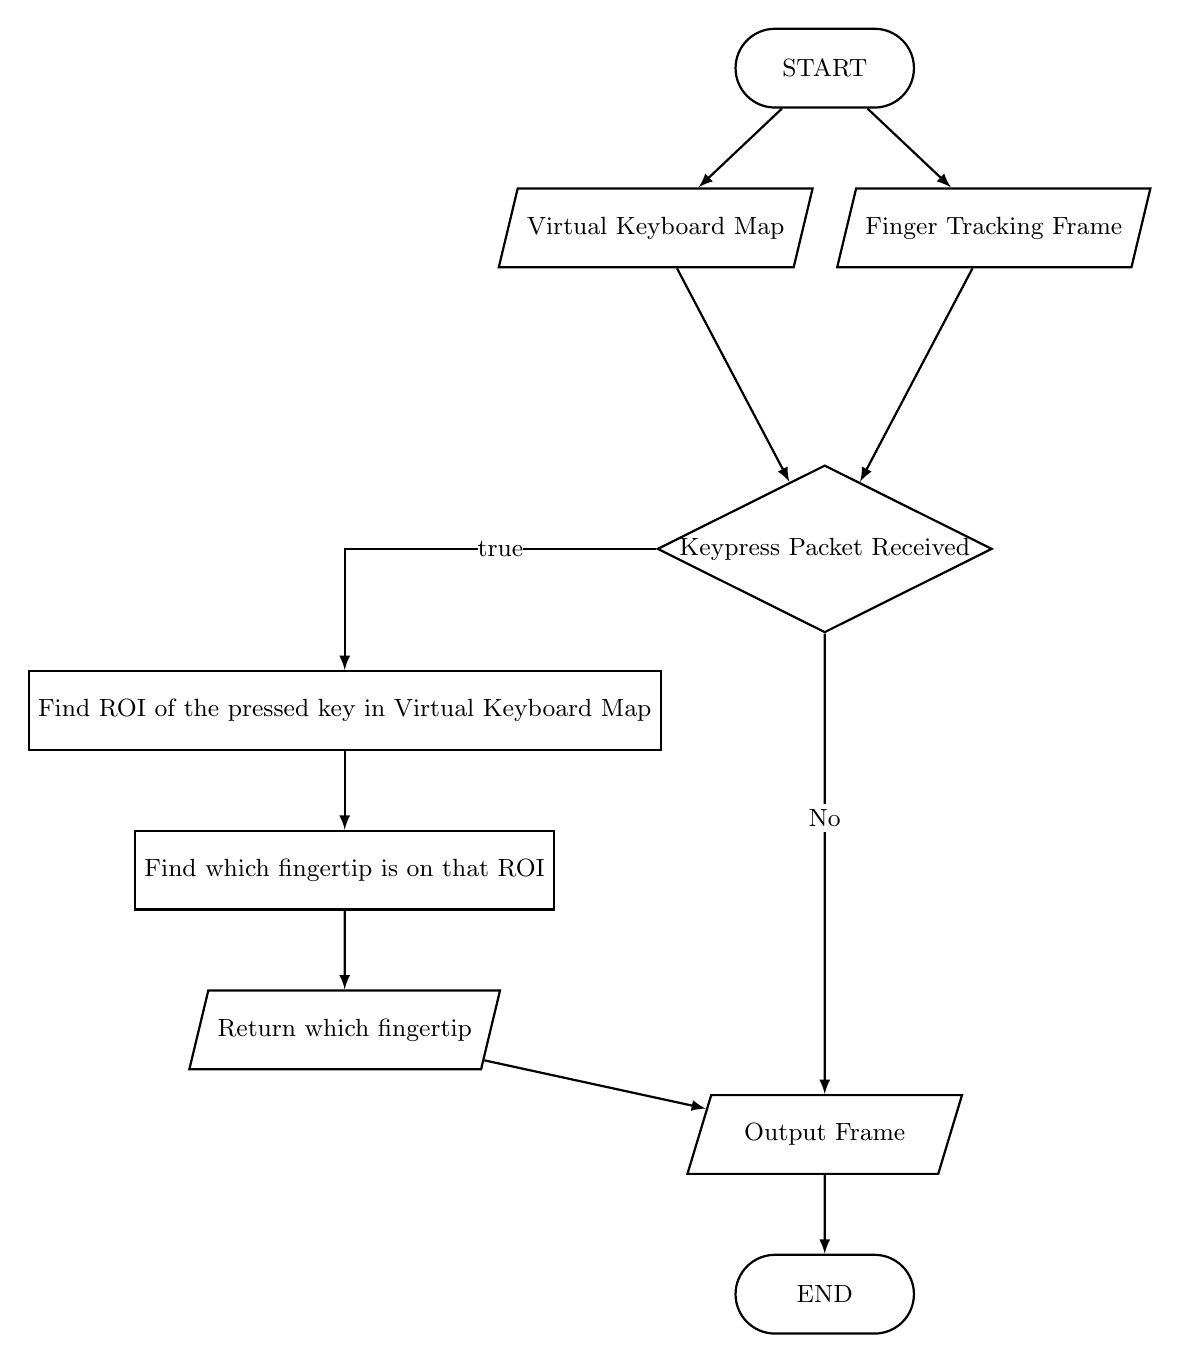
\begin{tikzpicture}[font=\small,thick]
		\node[draw,
			rounded rectangle,
			minimum width=2.5cm,
			minimum height=1cm] (start) {START};

		\node[draw,
			trapezium,
			trapezium left angle = 65,
			trapezium right angle = 115,
			trapezium stretches,
			below left=of start,
			minimum width=3.5cm,
			minimum height=1cm
		] (map) {Virtual Keyboard Map};

		\node[draw,
			trapezium,
			trapezium left angle = 65,
			trapezium right angle = 115,
			trapezium stretches,
			below right=of start,
			minimum width=3.5cm,
			minimum height=1cm
		] (track) {Finger Tracking Frame};

		\coordinate (CENTER) at ($(map)!0.5!(track)$);

		\node[draw,
			diamond,
			aspect=2,
			below = 3cm of CENTER,
			minimum width=2.5cm,
			inner sep=0] (if-packet) {Keypress Packet Received};

		\node[draw,
			below left=of if-packet,
			minimum width=3.5cm,
			minimum height=1cm] (find-roi) {Find ROI of the pressed key in Virtual Keyboard Map};

		\node[draw,
			below=of find-roi,
			minimum width=3.5cm,
			minimum height=1cm] (find-finger) {Find which fingertip is on that ROI};


		\node[draw,
			trapezium,
			trapezium left angle = 65,
			trapezium right angle = 115,
			trapezium stretches,
			below=of find-finger,
			minimum width=3.5cm,
			minimum height=1cm
		] (return) {Return which fingertip};

		\node[draw,
			trapezium,
			trapezium left angle = 65,
			trapezium right angle = 115,
			trapezium stretches,
			below = 11cm of CENTER,
			minimum width=3.5cm,
			minimum height=1cm
		] (output) {Output Frame};

		\node[draw,
			below=of output,
			rounded rectangle,
			minimum width=2.5cm,
			minimum height=1cm] (end) {END};

		\draw[-latex] (start) edge (map)
		(start) edge (track)
		(track) edge (if-packet)
		(map) edge (if-packet)
		(find-roi) edge (find-finger)
		(find-finger) edge (return)
		(return) edge (output)
		(output) edge (end);

		\draw[-latex] (if-packet) -| (find-roi)
		node[pos=0.25,fill=white,inner sep=0]{true};

		\draw[-latex] (if-packet) edge node[pos=0.4,fill=white,inner sep=2pt]{No}(output);

	\end{tikzpicture}
	\caption{Flowchart of the overall flow}
	\label{fig:metho-algo-integration}
\end{figure}

\subsubsection{Find ROI of the pressend key in Virtual Keyboard Map}
Since there is a known color-key mapping based on the Virtual Keyboard Map, the
algorithm will find the correct color to search for based on the received
keypress packet. This color is isolated from the Virtual Keyboard Map, and the
region of interest and its coordinates are obtained. The edges of this ROI will
then be obtained by finding its contours. The specific implementation of this is
explained in Section~\ref{section:metho-algo-key-contours}.

The coordinate system will have its origin at the top left, starting at 0, 0.
Going to the right increases the value of the x-axis, and going to the bottom
increases the value of the y-axis. This will result in a coordinate system that
only has positive values with each value corresponding to a pixel.

The expected output of this is four sets of pairs. Each pair corresponds to an
edge of the region of interest.

\subsubsection{Find which fingertip is on that ROI}
The Finger Tracking Frame will contain the pixel positions of each landmark of
the hand. For this step, the algorithm will find the landmark which is
positioned within the region of interest obtained from the previous step. This
will be done using a series of checks.

Each landmark's coordinates will be compared to the coordinates of the edges of
the ROI. A landmark will be determined as positioned within the ROI if all of the
following conditions are true:
\begin{enumerate}
	\item In the X axis, the landmark's coordinates is greater than one or both of
		the two coordinates found of the left side of the ROI
	\item In the X axis, the landmark's coordinates is less than one or both of
		the two coordinates found of the right side of the ROI
	\item In the Y axis, the landmark's coordinates is greater than one or both of
		the two coordinates found of the top side of the ROI
	\item In the Y axis, the landmark's coordinates is less than one or both of
		the two coordinates found of the bottom side of the ROI
\end{enumerate}

These conditions maximize the total area of the ROI and is not strict about
exact accuracy. In essence, these conditions will create a perfectly rectangular
box that contains the quadrilateral formed by the four points from the previous
step.

\subsubsection{Return which fingertip}
The landmark will then be used to determine which specific finger corresponds to
the keypress. Figure~\ref{fig:metho-algo-integration-landmarks} shows each
possible landmark that may be returned from the previous step. This step will
then return the name of the landmark, up until the first underscore. As an
example, if the landmark found is \texttt{MIDDLE\_FINGER\_TIP}, this step will
return \texttt{MIDDLE} denoting that the middle finger is the finger that
corresponds with the keypress. In addition, the specific hand will also be
returned as one of two strings, \texttt{Left} and \texttt{Right}, since
this information is also bundled together with the landmarks.

\begin{figure}[H]
	\centering
	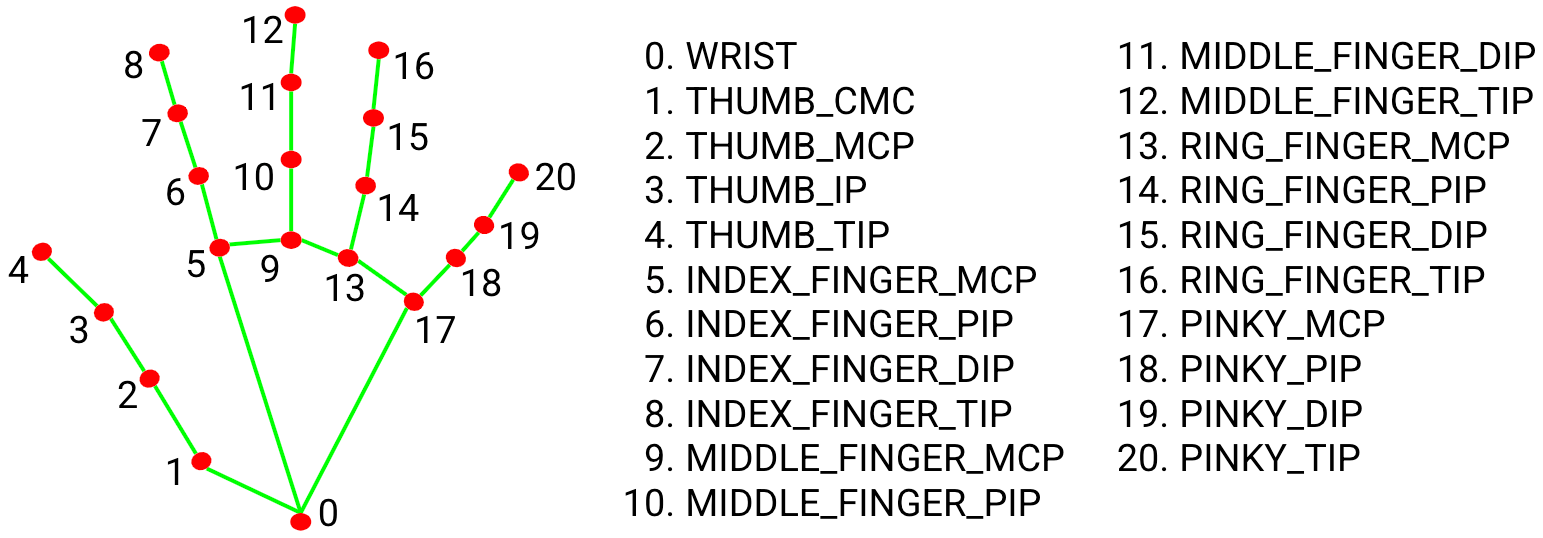
\includegraphics[width=0.6\textwidth]{hand-landmarks.png}
	\caption{Hand landmarks that may be returned by the algorithm. Reproduced from \fullcite{mediapipe-hands}}.
	\label{fig:metho-algo-integration-landmarks}
	\centering
\end{figure}

\subsection{Implementation}
\label{section:metho-algo-implementation}
The previously discussed algorithms will be implemented using Python. The
Keyboard Detection, and Mapping Algorithm in
Section~\ref{section:metho-algo-keyboard} will be implemented as a separate
submodule in Python using OpenCV.\@The Finger Detection, and Tracking Solution
in Section~\ref{section:metho-algo-finger} will be consumed using the prebuilt
Python package offered by the MediaPipe team. Finally, the integration of the
two will be done as another separate submodule in Python.

\section{Trainer}

\subsection{Typing Test Sequences}
Typing test sequences are strings that will be used in testing the user in their
ability to type. The test sequences that will be used in the trainer will come
from text found in the public domain obtained from Project Gutenberg and the
Internet Archive. Sentences will be isolated from these text and used as test
sequences if they fit a criteria.

The criteria for choosing test sequences is as follows: (1) $\approx80\%$ of the
characters in the keyboard is present in a test sequence. (2) The number of
words in a test sequence do not exceed 25. (3) Numbers and punctuations should
be present in at least $\approx30\%$ of the total test sequences.

There will be a total of 10 test sequences that will be gathered. An example
test sequence is ``What of it, if some old hunks of a sea-captain orders me to
get a broom and sweep down the decks?'' from Moby Dick by \cite{moby-dick}. The
9 other test sequences can be found in the appendix.

\subsection{UX/UI design and Front-end development for the touch typing trainer}
\subsubsection{Design}
This design will be based on other type tests such as Monkeytype
\parencite{bartnik2021}, and Keybr \parencite{keybr}, with additional components
for showing real-time finger-key identification and mapping.
Figure~\ref{fig:ui-test} and \ref{fig:ui-stat} illustrates the two main pages of
the design. Additional screens, such as historical statistics, in-platform
tutorial, and a written guide are shown in the appendix.

\begin{figure}[H]
	\centering
	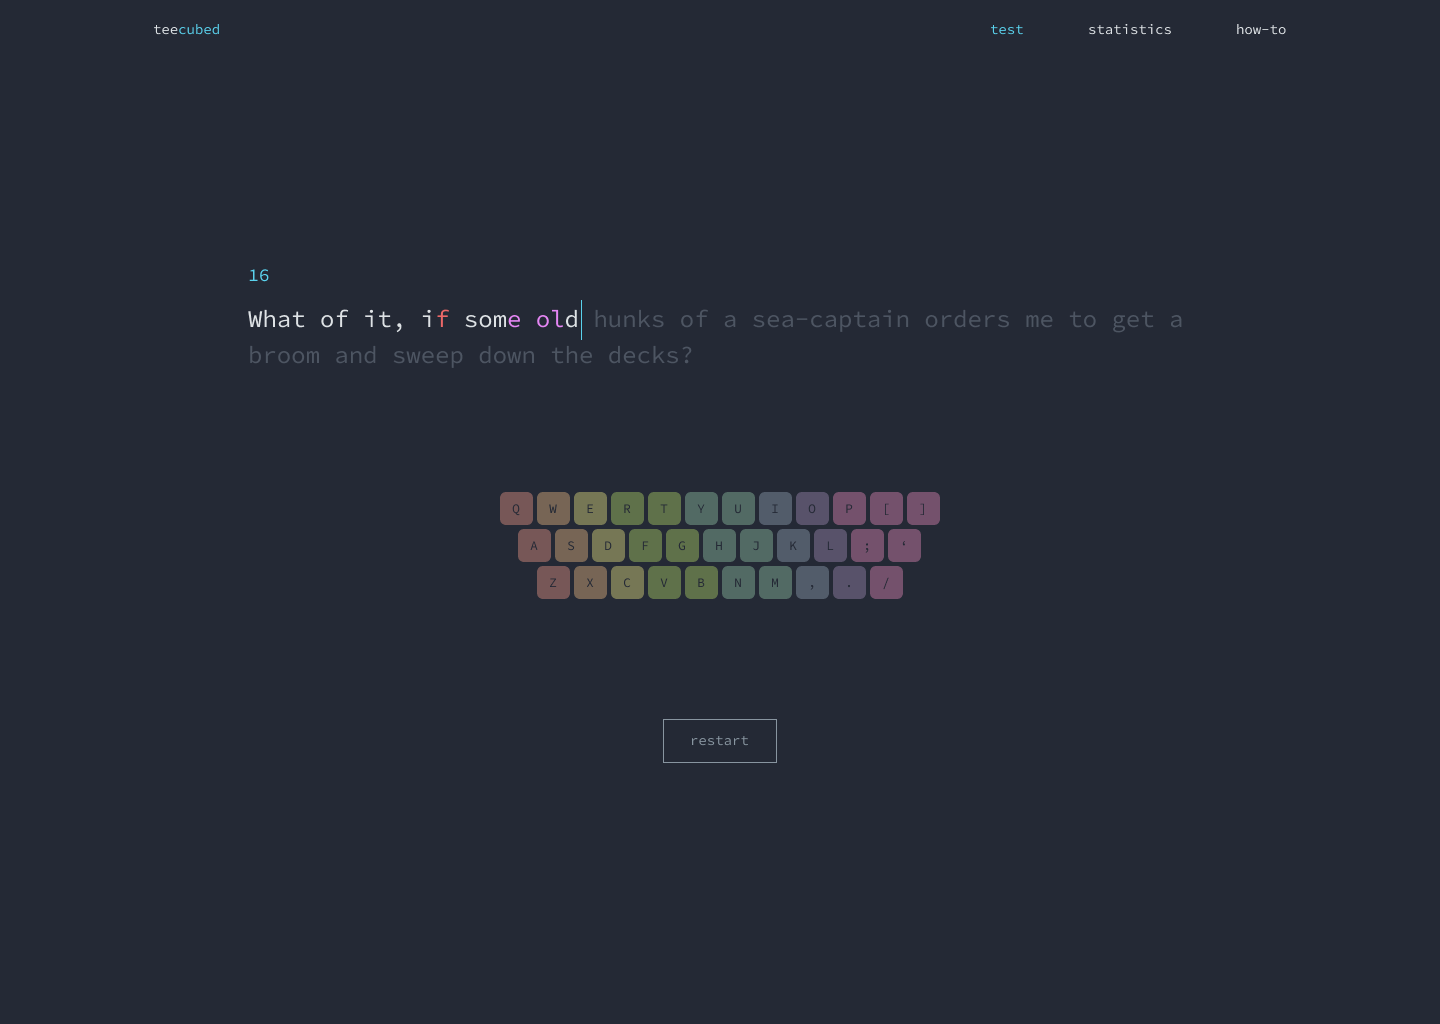
\includegraphics[width=0.8\textwidth]{ui-test.png}
	\caption{Test screen of the front-end design}
	\label{fig:ui-test}
	\centering
\end{figure}

Figure~\ref{fig:ui-test} has four main components. From the top, the first
component is the navigation bar. This directs the user to the different pages
within the website. The second component in the upper left displays the number
of remaining words to be typed. This is 16 in the example. Below that is the
test sequence. This shows the user what characters to type, and highlights
mistakes in two distinct colors. Red if the character pressed was incorrect and
purple if the character typed was correct, but the finger used to type it is
wrong. The last main component in this screen is the keyboard that illustrates
the correct finger positioning, with each finger corresponding to a different
color.

\begin{figure}[H]
	\centering
	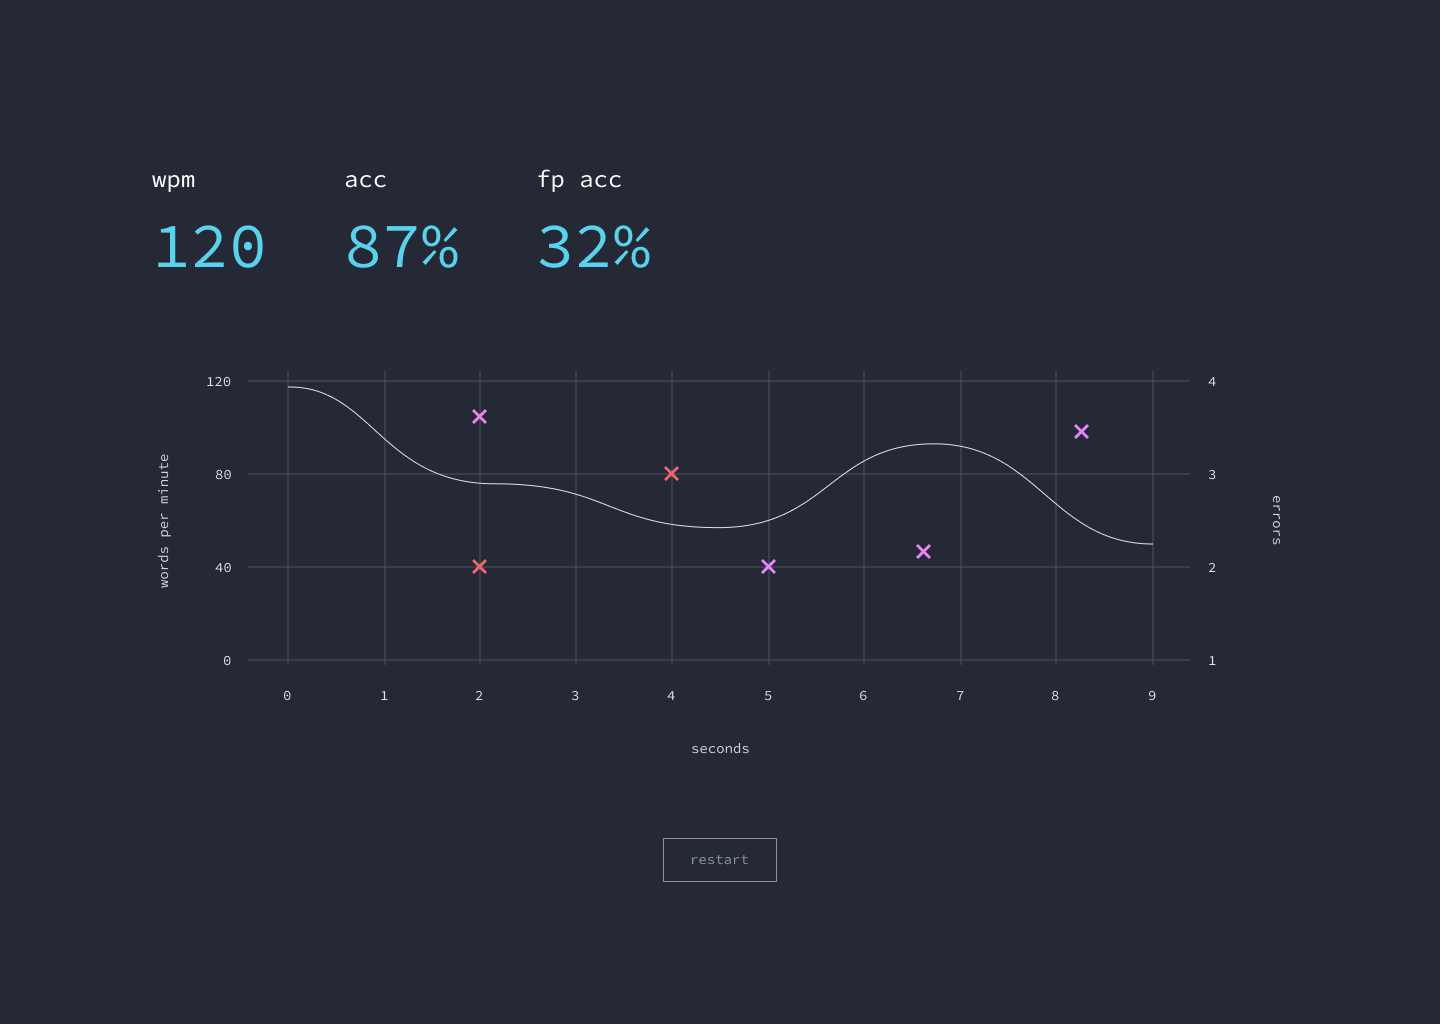
\includegraphics[width=0.8\textwidth]{ui-stats.png}
	\caption{Statistics screen of the front-end design}
	\label{fig:ui-stat}
	\centering
\end{figure}

Figure~\ref{fig:ui-stat} has two main components. The first component at the top
shows the three major statistics for the typing test: Words per minute,
Accuracy, and Finger placement accuracy. Finger placement accuracy will be
explained in Section~\ref{label:metric}. The component below the statistics is a
graph plotting the major statistics of the user in time. This includes when the
user made the mistake and when the user slowed down, or increased their speed.

\subsubsection{Implementation}
The design will be created in Figma and the front-end will be web based.The
framework the front-end will be developed in will be Svelte, due to its
community resources, performance, and the researcher's familiarity with the
framework. The front-end will serve as a display for the information and the
interface which the user interacts and inputs information into the trainer. No
calculation will be done within the front-end.

\subsection{Back-end development of a touch typing trainer using the program created
	in \ref{section:metho-algo} and the experimental setup identified in
	\ref{section:metho-setup}}

The back-end will handle all of the computation for the trainer---mainly
finger-key identification. The backend will also handle authentication and data
storage.

The back-end will expose a REST API. This is a type of application programming
interface (API) that conforms to the REST architectural style. One key
characteristic of the this style is its statelessness and cacheable data
\parencite{rest}. This will be implemented using Django, a Python REST API
framework.

\subsubsection{Finger-key Identification}
The submodule that integrates all of the sub algorithms will be called within
the framework. The framework will then respond to requests for finger-key
identification using this submodule. This will allow the back-end to expose its
finger-key identification abilities and allow the front-end to use this data for
the trainer.

\subsubsection{Authentication}
The core authentication system will rely on JSON Web Tokens (JWTs) . According
to \cite{jwt}, ``JSON Web Token (JWT) is a compact, URL-safe means of
representing claims to be transferred between two parties.'' This allows for a
user to claim that they are that specific user securely as the claim is
cryptographically signed. For the backend of the trainer, the JWT will be signed
using a secret and it will be encoded in HMAC SHA256.

\subsubsection{Data Storage}
The trainer will store all of the data in a relational database using
PostgreSQL.\@This specific technology was chosen due to its maturity, community,
and industry recommendations and the researchers' familiarity with the
technology.

\subsection{Testing of finger-key identification and mapping accuracy}

There will be 15 videos of the researcher performing the typing test sequences.
The researcher will then manually perform finger-key identification for all key
presses present in the video. The finger-key identification submodule will then
perform the same process for the same videos. The accuracy of the submodule will
then be obtained by identifying which of its identification is incorrect, based
on the manual identification.

\section{Metric}
\label{section:metric}

There will be two total metrics obtained pertaining to finger and key mapping.
The first will be per test sequence, and the second will be per key.

%% 4. Finger Placement Keyboard Typing Metric Development
%%     1. Determine if the metric is for individual key presses or for the whole typing sequence or both.
%%     2. Evaluate which variables need to be taken into account for the metric depending on (5.a):
%%         1. Actual Finger Used
%%         2. Correct Finger to be Used
%%         3. Specific key pressed
%%         4. Number of keys pressed with the correct fingers
%%         5. Number of keys pressed with the wrong fingers

\newpage
\printbibliography[heading=bibintoc,title={References}]{}

\end{document}
